%  LaTeX support: latex@mdpi.com
%  In case you need support, please attach any log files that you could have, and specify the details of your LaTeX setup (which operating system and LaTeX version / tools you are using).

%=================================================================

% LaTeX Class File and Rendering Mode (choose one)
% You will need to save the "mdpi.cls" and "mdpi.bst" files into the same folder as this template file.

%=================================================================

\documentclass[jmse,article,submit,moreauthors,pdftex,12pt,a4paper]{mdpi} 
%--------------------
% Class Options:
%--------------------
% journal
%----------
% Choose between the following MDPI journals:
% actuators, administrativesciences, aerospace, agriculture, agronomy, algorithms, animals, antibiotics, antibodies, antioxidants, appliedsciences, arts, atmosphere, atoms, axioms, behavioralsciences, bioengineering, biology, biomedicines, biomolecules, biosensors, brainsciences, buildings, cancers, catalysts, cells, challenges, chemosensors, children, chromatography, climate, coatings, computation, computers, cosmetics, crystals, dentistryjournal, diagnostics, diseases, diversity, econometrics, economies, education, electronics, energies, entropy, environmentalsciences, fibers, foods, forests, futureinternet, galaxies, games, genes, geosciences, healthcare, humanities, informatics, information, inorganics, insects, ijerph, ijfs, ijms, ijgi, jcdd, jcm, jdb, jfb, joi, jlpea, jmse, jpm, jrfm, jsan, land, laws, life, lubricants, machines, marinedrugs, materials, mathematics, medicalsciences, membranes, metabolites, metals, microarrays, micromachines, microorganisms, minerals, molbank, molecules, nanomaterials, nutrients, optics, pathogens, pharmaceuticals, pharmaceutics, pharmacy, plants, polymers, processes, proteomes, publications, religions, remotesensing, resources, risks, robotics, sensors, socialsciences, societies, sports, sustainability, symmetry, systems, technologies, toxics, toxins, vaccines, veterinarysciences, viruses, water
%---------
% article
%---------
% The default type of manuscript is article, but could be replaced by using one of the class options: 
% article, review, communication, commentary, letter, bookreview, correction, addendum, editorial.
%----------
% submit
%----------
% The class option "submit" will be changed to "accept" by the Editorial Office when the paper is accepted. This will only make changes to the frontpage (e.g. the logo of the journal will get visible), the headings, and the copyright information. Journal info and pagination for accepted papers will also be assigned by the Editorial Office.
%------------------
% moreauthors
%------------------
% If there is only one author the class option oneauthor should be used. Otherwise use the class option moreauthors.
%---------
% pdftex
%---------
% The option "pdftex" is for use with pdfLaTeX only. If eps figure are used, use the optioin "dvipdfm", with LaTeX and dvi2pdf only.

%=================================================================

\setcounter{page}{1}
\lastpage{x}
\doinum{10.3390/------}
\pubvolume{xx}
\pubyear{2013}
\history{Received: xx / Accepted: xx / Published: xx}
%------------------------------------------------------------------
% The following line should be uncommented if the LaTeX file is uploaded to arXiv.org
%\pdfoutput=1

%=================================================================

% Add packages and commands to include here
% The amsmath, hyperref, caption, float and color packages are already included.
%\usepackage{amssymb}
\usepackage{graphicx}
%S\usepackage{cite}
%\usepackage{subfigure,psfig}

%=================================================================

% Full title of the paper (Capitalized)
\Title{The ADCIRC Surge Guidance System}

% Authors (Add full first names)
\Author{Jason Fleming $^{1,}$*, Janelle Reynolds-Fleming $^{1}$ and Rick Luettich $^{2}$}

% Affiliations / Addresses (Add [1] after \address if there is only one affiliation.)
\address{%
$^{1}$ Seahorse Coastal Consulting, 3103 Mandy Ln, Morehead City, North Carolina, USA\\
$^{2}$ Institute of Marine Sciences, University of North Carolina at Chapel Hill, 3431 Arendell St., Morehead City, North Carolina 28557, USA}

% Contact information of the corresponding author (Add [2] after \corres if there are more than one corresponding author.)
\corres{jason.fleming@seahorsecoastal.com, +1 252 726 6323}

% Abstract
\abstract{The ADCIRC Surge Guidance System (ASGS) is 
a real time software system for coastal ocean modeling that uses the 
ADCIRC coastal circulation model with optional coupling to the SWAN 
wave model. Initial development occurred in the aftermath of 
hurricane Katrina in 2006, and reliability, performance, and 
flexibility were key objectives. The ASGS has been applied 
successfully in many real time events, most recently including 
hurricanes Irene, Isaac, and Sandy as well as the 2010 Deepwater 
Horizon event. It is the first freely available real time automated 
coastal modeling system that is relocatable as well as portable 
across computing platforms. All the components of the system are 
open source and available for inspection, collaborative development 
and widespread independent application.}

% Keywords: add 3 to 10 keywords
\keyword{adcirc; storm surge; automation; real time; visualization}

% The fields PACS and MSC may be left empty or commented out if not applicable
%\PACS{}
%\MSC{}

\begin{document}

%%%%%%%%%%%%%%%%%%%%%%%%%%%%%%%%%%%%%%%%%%
%%%%%%%%%%%%%%%%%%%%%%%%%%%%%%%%%%%%%%%%%%

\section{Introduction}


Over the course of time, resource allocation for numerical storm 
surge calculations evolved on two separate tracks: simulations that 
were meant to be used operationally for emergency management, and 
those that were meant to be used in an offline design study. 
Computational resource allocation for real time storm surge 
applications has historically been far lower than in design studies 
and other non-real time applications. 

This bimodal distribution of resource requirements was strongly 
evident during the approach and landfall of hurricane Katrina on the 
northern Gulf coast of the US in 2005. The official storm surge 
forecasts that were produced in real time for Katrina using SLOSH 
contained a lower level of resolution and far lower computational 
resource allocation than the concurrent levee redesign project for 
southern Louisiana using ADCIRC and a high resolution input data set.

As a result of the desire for enhanced resolution and detail in real 
time guidance in the aftermath of Katrina, there was strong 
motivation to bring the computational resources of a design study to 
bear in real time. The ADCIRC Surge Guidance System (ASGS) was 
conceived at that time as a way to run the ADCIRC coastal ocean and 
storm surge model in real time in the event of a tropical cyclone 
threat. 

This paper on the ASGS updates our previous paper on the same 
subject \cite {FlemingJG2008} and describes the challenges 
associated with running such a model in real time; the technical 
approaches that were used in the design of the ASGS, and a survey of 
recent results. 

%%%%%%%%%%%%%%%%%%%%%%%%%%%%%%%%%%%%%%%%%%

\subsection{Literature Review}

A significant number of other researchers have produced automation 
software for coastal ocean models. As the technology supporting 
numerical storm surge calculations has developed, the value of the 
predictions for real time emergency response became. The first 
attempt to apply an existing coastal model in a real time context 
was the SLOSH model \cite{JelesnianskiCP1992}. The SLOSH model
requires minimal computational resources (running on a desktop
computer) and is thus able to complete forecast ensembles consisting
of hundreds of possible variations in only a few minutes.

More recently, several pilot projects have been developed to run a 
full scale ADCIRC model in real time to provide guidance for 
emergency managers. The first of these was the Southeast Coastal 
Ocean Observing and Prediction (SCOOP) system. This collaborative 
system relied on a geographically dispersed chain of contributors 
whose real time contributions to the guidance process were linked 
via Local Data Manager (LDM) from Unidata \cite {RamakrishnanL2006}. 
This SCOOP System represented an experimental cyberinfrastructure 
approach to distributed computation for storm surge prediction along 
the North Carolina Coast. It used ADCIRC for storm surge, and a 
separate Holland\cite{HollandGJ1980} symmetric vortex model for 
meteorological forcing based on the National Hurricane Center's 
forecast advisories. Large scale high performance computing (HPC) 
resources were obtained opportunistically using the Globus Toolkit, 
and files were transferred via GridFTP.  

Separately from the SCOOP System, the North Carolina Forecast System 
(NCFS) \cite{MattocksC2006} was also developed for the North 
Carolina coastline. It included a new asymmetric vortex model for 
production of meterological forcing data from National Hurricane 
Center Forecast Advisories and also used ADCIRC for storm surge 
computations. This system made use of different modes of operation, 
including background mode (tides only), nowcast event mode and 
forecast event mode mode in the event of a tropical cyclone. 

A relocatable ADCIRC automation system for the US Navy was recently 
developed \cite{ChuP2009} using a powerful template approach for 
constructing input files; this technique was later adopted in the 
design of the ASGS. The US Navy system used a toolbox approach that 
would allow simulations to be run in an automated or manual way. It 
divided up programs into five modules as follows: (1) system set up; 
(2) data acquisition; (3) model configuration; (4) model run status; 
and (5) product generation and dissemination. The toolbox even 
included a novel MeshGUI program that could be used by the operator 
to rapidly construct a new mesh in a short period of time if one was 
not already available for the area of interest. 

As stated previously, hurricane Katrina was the catalyst for the 
development of the Lake Pontchartrain Forecast System (LPFS) for the 
New Orleans District of the US Army Corps of Engineers \cite 
{FlemingJG2008}. The original target region was the south shore of 
Lake Pontchartrain (just to the north of the city of New Orleans) in 
Louisiana, USA. This location was selected because the Corps of 
Engineers had installed movable surge protection gates at the ends 
of the 17th St, Orleans Ave, and London Ave canals, which drain 
rainwater from the city. At that time, the surge gates were operated 
by cranes that could not be used in high winds; as a result, 
guidance on both the timing and magnitude of both winds and surge 
were important.

The original LPFS (the direct ancestor of the ASGS described here) 
did not include tidal forcing, river forcing, or wave coupling, and 
only generated simple hydrographs and wind speed plots for those 
three locations in real time. After its introduction in 2006 and 
continued development thereafter, the system was renamed the ADCIRC 
Surge Guidance System in 2009 to reflect its expansion of 
application beyond Lake Pontchartrain. 

The following section describes the evolution of the system from
its relatively limited form as the LPFS to the more flexible and 
powerful ASGS.

%%%%%%%%%%%%%%%%%%%%%%%%%%%%%%%%%%%%%%%%%%%%%%%%%%%%%%%%%%%%%%%%%
%%%%%%%%%%%%%%%%%%%%%%%%%%%%%%%%%%%%%%%%%%%%%%%%%%%%%%%%%%%%%%%%%
\section{Methods}

The design guidelines and workflow structure of the ASGS have developed 
according to the needs of emergency managers and official decision
makers as detailed in the following sections. 

%%%%%%%%%%%%%%%%%%%%%%%%%%%%%%%%%%%
%%%%%%%%%%%%%%%%%%%%%%%%%%%%%%%%%%%
\subsection{Design Considerations}

The hurricane seasons of 2006 and 2007 after the initial deployment 
of the LPFS were relatively quiet for the US in the Gulf of Mexico. 
However, the following season (2008) saw the landfall of hurricanes 
Gustav and Ike in quick succession as shown in Figure \ref 
{fig:hurricanes_2008}.

%    4   A T L A N T I C    H U R R I C A N E S 
\begin{figure}[t]
  \centering
  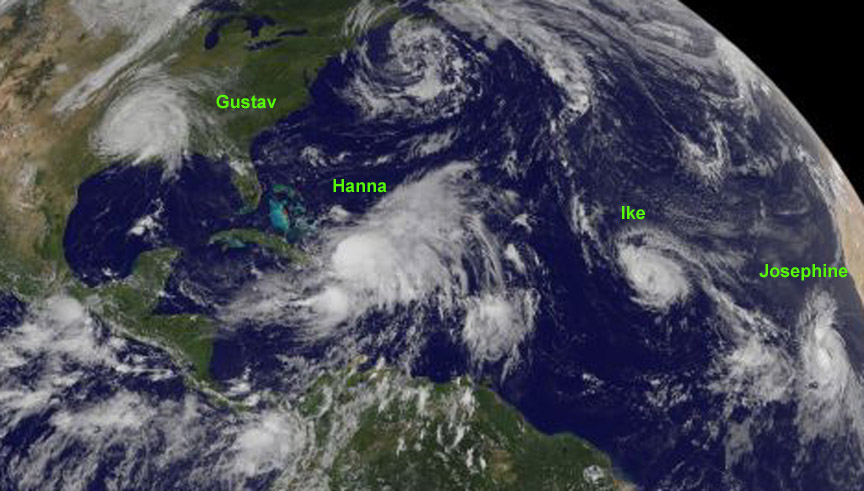
\includegraphics[width=0.9\textwidth]{4ATLHurricanes2008}\\
  \caption{Gustav and Ike made landfall on US shores in the Gulf of Mexico in 2008.}
  \label{fig:hurricanes_2008}
\end{figure}

During Gustav's evolution and approach, interaction with official 
decision makers made it clear that they had a strong need for real 
time ADCIRC guidance for many geographical areas beyond those 
originally selected. However, at that time the LPFS was a software 
automation with a geographically limited scope. A significant 
reprogramming effort was mounted in real time, between forecast 
advisories, to attempt keep up with the unanticipated expansion in 
demand for guidance in many other geographic locations. 

This ability to reprogram and adapt to changing needs in real time 
is a distinct advantage that the ASGS has over operational systems. 
As an aside, the word ``operational'' has a specific definition, 
meaning that the underlying model, input data, and automation 
software have been approved under a particular set of criteria and 
cannot be changed once they have been accepted for production. The 
ASGS, on the other hand, suffers no such limitations on its 
adaptability, and many changes can be made to the system, even in 
real time during the approach of a storm, to adapt it to the current 
circumstances. However, prior to the approach of hurricane Gustav in 
2008, such flexibility had not been a design goal.

Immediately following the landfall of hurricane Gustav in Louisiana 
in 2008, hurricane Ike traversed the Gulf, headed for a landfall in 
Texas. While Ike was having significant impacts in Louisiana, 
collaborators in Texas sought to run the ASGS for Texas as well, 
using a locally developed mesh and other input data on local high 
performance computing (HPC) resources. The resulting collaborative 
efforts highlighted the need for a system that was geographically 
relocatable and portable across computing platforms. The approach of 
hurricane Ike also highlighted the value of ongoing technical 
collaboration among regional participants that can share the 
technical and computational workloads during major events. 

In summary, after dealing with the challenges of the hurricanes Ike 
and Gustav during the 2008 season, it was found that (1) strong and 
growing demand existed for real time storm surge guidance using 
ADCIRC; (2) the narrow focus of the LPFS created gaps in 
relocatability, extensibility, portability, relocatability, and 
collaboration that would have to be closed in order to fulfill that 
demand. 

The methods that were applied during the expansion and 
generalization of that initial system are described in the following 
sections. 

%%%%%%%%%%%%%%%%%%%%%%%%%%%%%%
\subsection{Collaboration Strategy}

The selection of a collaboration strategy has a suprisingly strong 
influence on the quality and longevity of the underlying technology 
products. Collaboration has many advantages as well as pitfalls, and 
successful collaboration requires that the incentives of the 
participants be aligned and that each contributor maintain a focus 
on results rather than process. 

In order to illustrate the characteristics of different 
collaboration strategies that are commonly used when developing real 
time storm surge guidance system, three different collaboration 
strategies are described here. These three strategies are termed the 
``closed system'', the ``distributed chain'', and the ``regional 
team'' approach. Each of these are described below, along with their 
effects on development processes, real time operations, and 
technological vibrancy.

A so-called ``closed system'' is the result of a collaboration 
within a unified team of developers that takes responsibility for 
every aspect of the system and its operation: gathering of physical 
(e.g., bathymetry) data, construction of a meteorological model, 
offline validation, computational resource allocation, post 
processing, visualization, dissemination of output products to end 
users within the same organization, and the software automation to 
make the whole stack run in real time. Nearly all real time guidance 
systems for storm surge that have been detailed in the research 
literature were developed using this approach.

The advantages of a closed system are simplicity and control. 
Simplicity results from the need to only code for a single 
computational plaform with a narrow set of capabilites as required 
to satisfy the target audience. All other things being equal, simple 
systems are more reliable and easier to maintain than complex 
systems. Closed systems are also easier to control because they 
benefit from the availability of dedicated resources, including HPC 
resources, staff time, and a single chain of command with high level 
buy-in for the stated objectives of the real time guidance system.

The disadvantages of the closed system are expense, inflexibility, 
and insularity. Closed systems are relatively expensive because all 
research, development, maintenance, and operation costs must be 
borne by a single working group within an organization. New features 
and capabilities can only be produced as the time and budget of that 
group allows, and development of new capabilities must be balanced 
against the need to maintain and operate in production.

The final disadvantage of any closed system is insularity. The lack 
of technology sharing with other working groups, or applications for 
other projects or end users tends to limit the expansion of the 
technology to new areas, especially those outside the experience of 
the foundational team. 

In contrast, the second type of collaboration strategy, the 
``distributed chain'' approach, is the polar opposite of the closed 
system described previously. The distributed chain strategy starts 
by conceptually modularizing the overall functionality into discrete 
subsystems. The responsibility for development and real time 
operation of each subsystem is then distributed to separate 
organizations that are linked through the internet via a common data 
bus that allows them to build storm surge products in an assembly 
line fashion. For example, one organization may be run a numerical 
weather model, while another orgainzation sets up a surge model, 
with computational resources being offered by a third organization. 
The distributed chain approach was pioneered by the team that 
developed the SCOOP system and applied it to real time storm surge 
guidance for the North Carolina Coast. \cite{RamakrishnanL2006}

The advantages and disadvantages of the distributed chain system are 
mostly the inverse of the closed system. The advantages of the 
distributed chain are flexibility and vibrancy. Because of the 
open-participation philosophy and sharing of a common data bus, the 
barrier to entry of new participants and new ideas is low, and as a 
result such collaboration strategies attract new ideas and new 
participants easily.

The disadvantages of a distributed chain are complexity and lack of 
control: each time another institution or software system are 
included in the chain, the system becomes more complex and the 
number of potential points of failure increases. The increase in the 
number of failure points is particularly significant because the 
chain is only as strong as its weakest link. And because each link 
in the chain is operated independently, there isn't a single point 
of accountability for all of the participants.

Both closed systems and distributed chains face the burden of 
reinventing the wheel when implementing new features, and even 
issues of long term viability; these issues result from a lack of 
freely shared technology. Closed system technologies and the 
individual components of distributed chain systems are generally 
kept ``in-house'' and are not freely shared with other developers 
outside the organization. Even within a given team, staff turnover 
may create continuity issues. Furthermore, the products of these 
teams will continue to be available only from their original 
developers and only for as long as they are able to produce them, 
and the issues of insularity still apply to those technologies.

In order to combine the advantages of both the closed system and 
distributed chain approaches while avoiding their respective 
disadvantages, the ASGS has been developed using a regional team 
approach. Figure \ref{fig:regional_teams} illustrates the current 
roster of regional teams that develop and operate the ASGS. 

%    R E G I O N A L   T E A M S  
\begin{figure}[t]
  \centering
  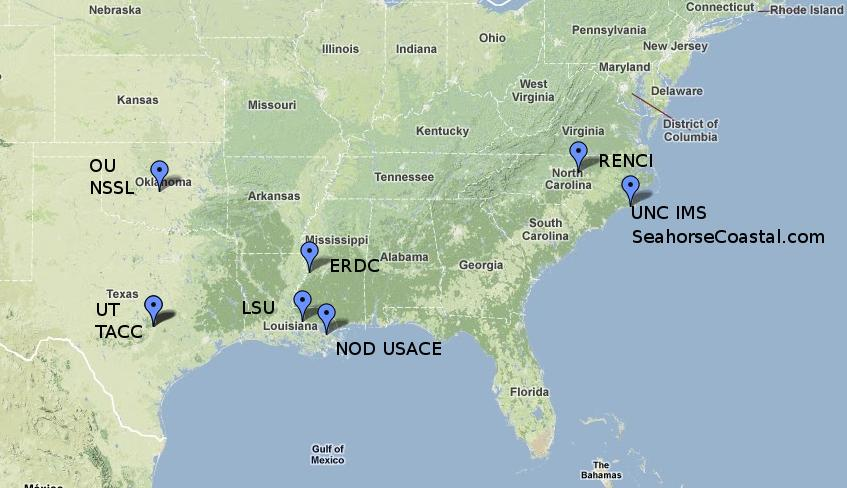
\includegraphics[width=0.8\textwidth]{regional_teams}\\
  \caption{A collaboration among self contained regional teams facilitates reliability as well as vibrancy.}
  \label{fig:regional_teams}
\end{figure}

Investigators at the University of North Caronlina at Chapel Hill 
Institute of Marine Sciences (UNC IMS) provides advocacy, visibility, 
credibility and thought leadership for the overall ASGS project. 

Seahorse Coastal Consulting has led the technical development and 
programming of the ASGS code since the project's inception in 2006. 
Furthermore, Seahorse Coastal Consulting also collaborates with UNC 
IMS to operate the ASGS for the New Orleans District of the US Army 
Corps of Engineers using HPC resources at the Engineering Research 
and Development Center (ERDC) to produce guidance for the Louisiana 
coast. Furthermore, Seahorse Coastal Consulting also collaborates with 
the Renaissance Computing Institute (RENCI) to produce guidance for 
the State of North Carolina using RENCI HPC resources. 

In addition to HPC resources and support, the Renaissance Computing 
Institute has also developed a series of novel cyberinfrastructure 
capabilities (including indexing, visualization and analysis) \cite 
{BlantonBO2012} that take advantage of the unique structure of the 
ASGS and its autonomous, replicated production of results. In 
addition, RENCI has also coordinated structured outreach with local 
emergency managers to collect feedback on the provision of storm 
surge information to improve the construction of output products and 
their dissemination \cite {LosegoJL2012}. 

The ASGS for North Carolina is further supported by teams at the 
University of Oklahoma (OU) and the National Severe Storms 
Laboratory (NSSL) with a hydrological model of eastern North 
Carolina that provides upstream river boundary conditions. The NSSL 
also aggregates the final results from the North Carolina ASGS with 
other meteorological and stream flow information into a 
password-protected web application called Coastal and Inland 
Flooding Observation and Warning (CIFLOW) \cite {VanCootenS2011} for 
officials within NOAA. The OU team has also contributed quantitative
skill assessments of ASGS results for past events in order to 
inform the future development of the system and its underlying 
models. \cite{DresbackKM2013}

The ASGS is also operated locally (and autonomously) by regional 
team members in Louisiana and Texas. The Louisiana team is based at 
Louisiana State University and operates the ASGS on HPC resources 
there, advising the Louisiana Governor's Office of Homeland Security 
and Emergency Preparedness (GOSHEP)  as well as numerous state and 
local agencies using generated results from their own instances of 
the ASGS when a tropical cyclone is threatening the Lousiana coast. 
Furthermore, the Louisiana team is also the developer of the Coastal 
Emergency Risks Assessment (CERA) web application that provides 
fully interactive map-based visualization of ASGS results for use by 
emergency managers and other officials in Louisiana.

The Texas team operates the ASGS for the Texas coast on HPC 
resources at the University of Texas \cite{DietrichJC2013} whenever 
a storm threatens the Texas coast. The Texas team advises the Texas 
State Operations Center (SOC), as well as other state and local 
emergency managment and National Weather Service (NWS) offices. 
Furthermore, the Texas team has developed locally appropriate 
visualization capabilities using the FigureGen software package, and 
was instrumental in the production of NSF-sponsored ASGS results for 
surface oil slick modeling during the Deepwater Horizon event in 
2010 \cite {DietrichJC2012}. 

In this regional team paradigm, all collaborators have full access 
to the entire software stack and all documentation, which is freely 
shared. In addition, each team has a responsibility to provide real 
time guidance only in their local area and the freedom to adapt and 
enhance the ASGS as needed to meet the needs of local officials. 
This approach distributes the workload of development and operation 
to a large group (as in the distributed chain approach) while 
maintaining strong accountability and results orientation as in the 
closed system approach. 

The regional team approach offers the flexibility and vibrancy of 
the distributed chain, since the existing technology is freely 
shared among participants, enabling new participants to get up to 
speed quickly while existing participants benefit from sharing new 
features. It also solves the weakest link and accoutability issues 
inherent in the distributed chain approach, since each regional team 
operates independently in a self-contained way during a real time 
event, and each team is subject to a single local chain of command and 
coordination in real time.

The expense of the regional team approach is relatively low, 
particularly for new participants, because the burden of ongoing 
maintenance efforts and new feature development is distributed among 
all participants, while the benefits of those efforts are shared by 
all, preventing any regional team from having to reinvent the wheel. 
However, in order for the benefits of technology sharing to accrue, 
a central figure must take responsibility for coordinating the 
efforts of the various teams, integrating disparate features 
developed by different regional teams, developing new features in 
the underlying numerical models to support new capabilities in the 
software automation system, writing or aggregating documentation, 
ensuring continuity, and providing training and capacity building. 
Seahorse Coastal Consulting serves in this central supporting role, 
developing the ASGS documentation, conducting training seminars, and 
providing the general technical cohesion that facilitates the 
merging of new features back into a unified technology stack that 
benefits all participants. 

The final and perhaps most important advantage of the regional team 
collaboration strategy is that it dramatically enhances the 
likelihood that dedicated access to shared HPC resources will be 
granted for use in real time storm surge computations. Regional 
shared-resource HPC centers have an inherent incentive to provide 
resources to support real time modeling for a current event that is 
directly relevant to their region, and a strong disincentive to 
provide resources for events that are not locally relevant. For 
example, an HPC center on the Atlantic coast is not likely to grant 
dedicated real time access to their HPC resources for a storm that 
is threatening the Gulf coast, and vice versa. But an HPC center in 
any particular state is almost certain to grant dedicated access to 
compute guidance for a storm that will make landfall in that state. 
This alignment of incentives between an HPC center and its 
corresponding regional ASGS team greatly simplifies and facilitates 
dedicated access to HPC resources, and in our experience this 
advantage should not be underestimated. 

%%%%%%%%%%%%%%%%%%%%%%%%%%
\subsection{Reliability}

Speed and accuracy are useless if guidance cannot be produced 
because of software or hardware issues. A client that has scheduled 
an early morning briefing with high level officials must have 
guidance available for the brief, and even accuracy considerations 
take a back seat to the absolute requirement that results be 
available as scheduled. 

When designing for reliability, the two most valuable tools are 
simplicity and self-healing. Of those two, simplicity is the most 
important design consideration for reliable operation. A conceptual 
overview of the ASGS workflow that illustrates its relative 
simplicity is shown in Figure \ref{fig:asgs_overview}.

%    A S G S   O V E R V I E W   F L O W C H A R T
\begin{figure}[t]
  \centering
  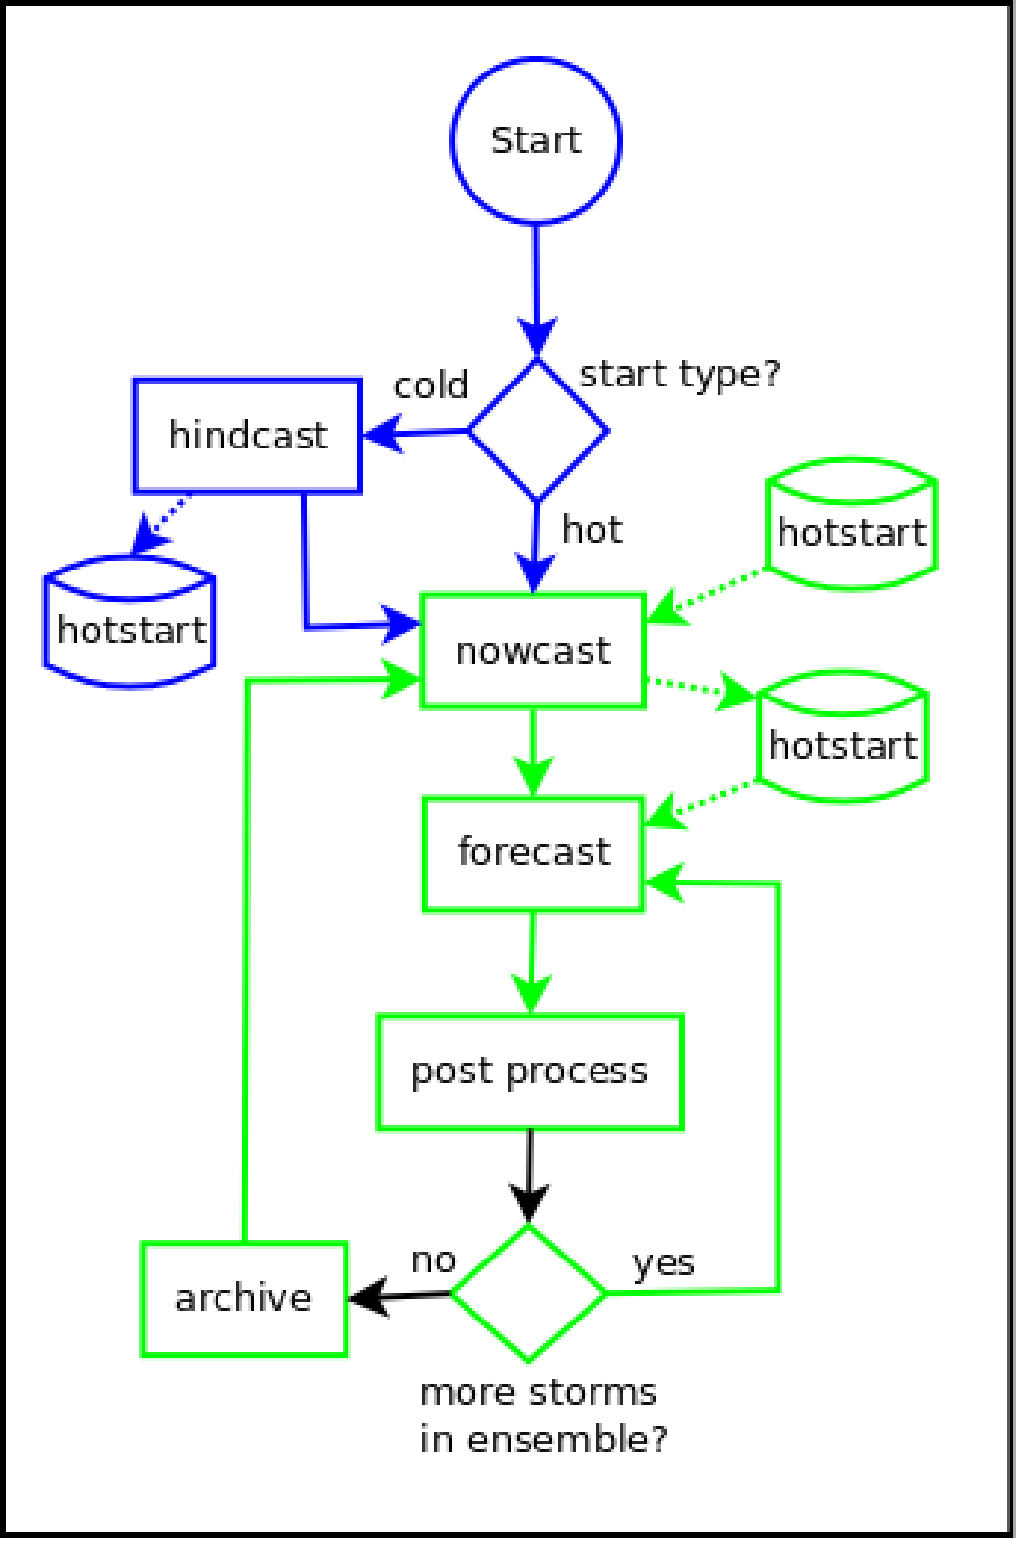
\includegraphics[width=0.5\textwidth]{asgs_overview_color}\\
  \caption{The architecture of the ASGS is conceptually simple and mainly consists of a nowcast/forecast loop coded as a single shell script.}
  \label{fig:asgs_overview}
\end{figure}

The core of the ASGS is the nowcast/forecast loop, as shown in green 
in Figure \ref{fig:asgs_overview}. Each time the externally supplied 
meteorological forcing is updated (e.g., whenever the National 
Hurricane Center issues a new advisory) the ASGS conducts a new 
nowcast to update the state of the solution from where it left off 
at the end of the previous nowcast to the current state at the start 
of the new forecast period. It causes the underlying physical model 
(ADCIRC or ADCIRC+SWAN) to record the current solution state in 
hotstart files at that point for use in starting one or more 
forecasts and for starting the next nowcast cycle. 

Once the forecast phase is complete, post processing and archiving 
of results proceed automatically, and the ASGS returns to the 
nowcast phase, waiting for new meteorological forcing data to become 
available. This nowcast/forecast loop is the core of the ASGS, and 
for the sake of simplicity this core functionality is implemented as 
a single shell script. This implementation provides a clean, 
comprehensible, and approachable superstructure that modularizes all 
complex processing into subprograms for tasks such as data 
transmittal, job handling, post processing, visualization, and 
archiving as shown in Figure~\ref{fig:asgs_structure}.

%    A S G S   S T R U C T U R E   D I A G R A M 
\begin{figure}[t]
  \centering
  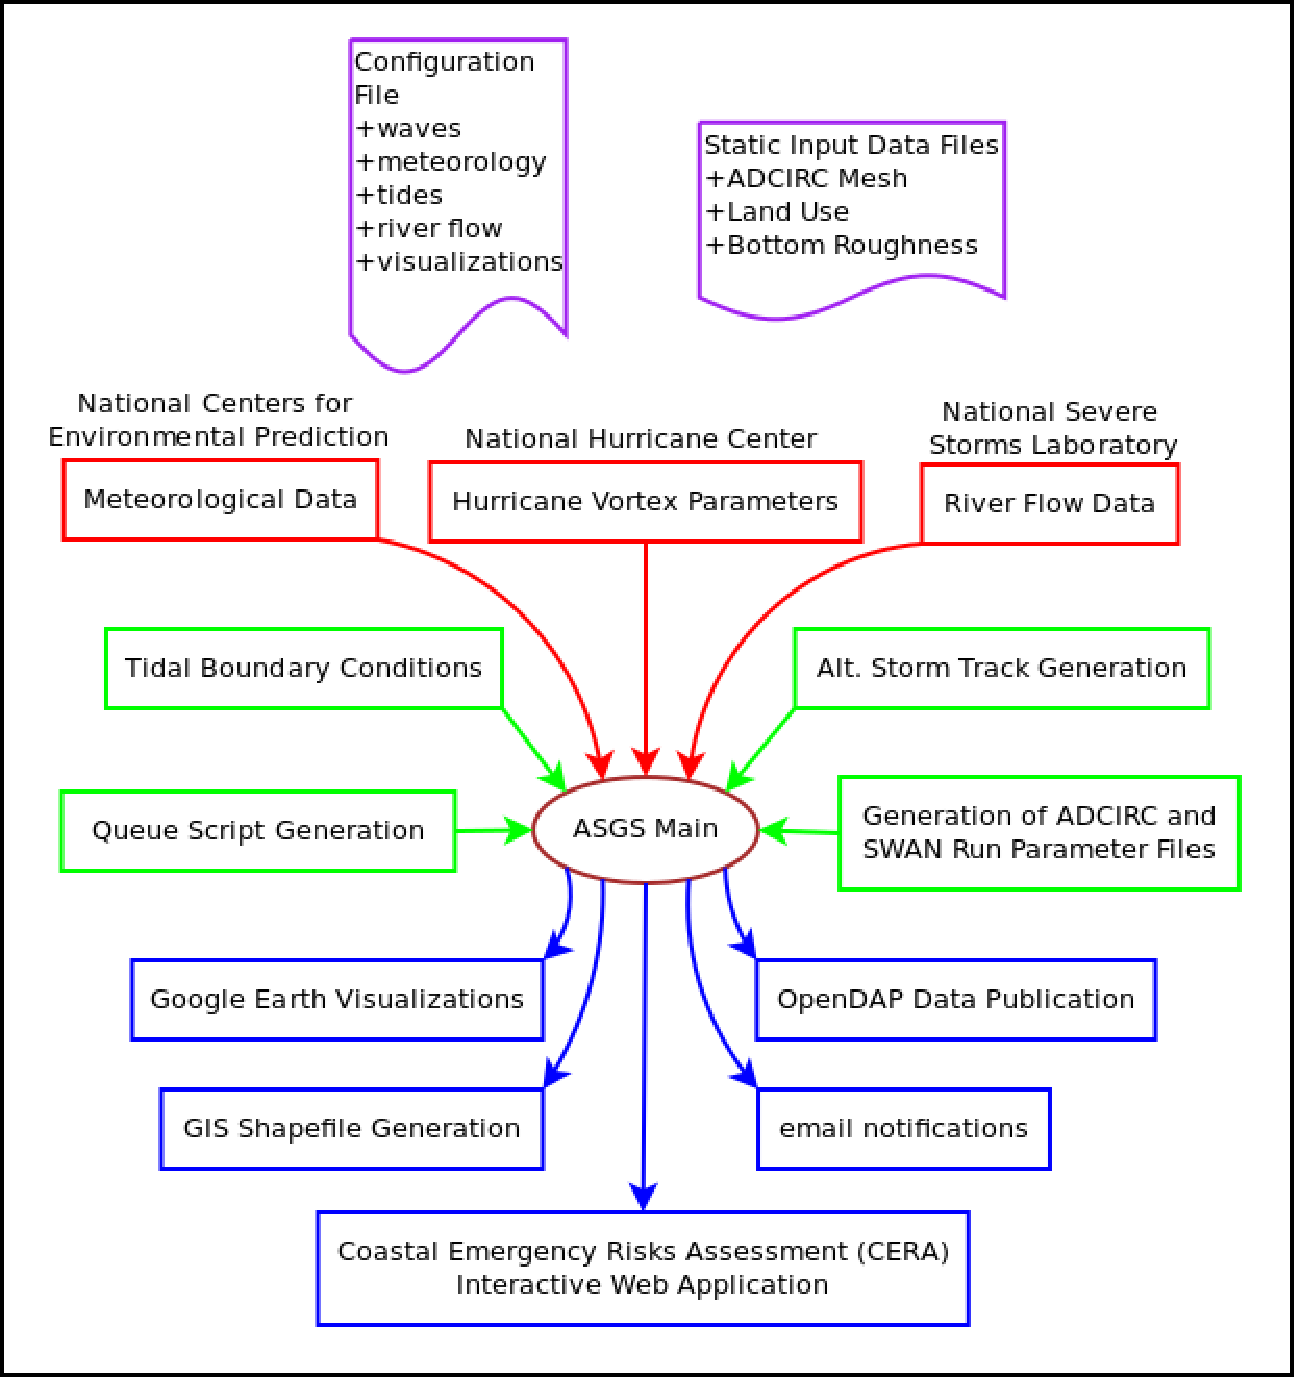
\includegraphics[width=0.8\textwidth]{asgs_structure_color}\\
  \caption{The ASGS is implemented as a core shell script with specialized subprograms that perform complex tasks.}
  \label{fig:asgs_structure}
\end{figure}


As a result of this architecture, starting up the ASGS is simply a 
matter of executing the core shell script. All the components of the 
ASGS are self-contained on a particular computing resource. 
Furthermore, if more than one copy of the ASGS is needed (for 
example, if reliability considerations require that guidance is also 
produced on a second machine for redundancy), starting up another 
instance is as easy as executing the core shell script a second time.

Self-checking is the second most important aspect for achieving 
reliable operation. The modular approach of the ASGS---where the 
main nowcast/forecast loop is coded as central shell script with all 
complex processing occurring in subprograms---provides a built-in
exception handling capability. 

For example, each subprogram was designed with pervasive error 
checking, consistency checking, and sanity checking to detect errors 
and anomalies in its own operations. Wherever possible, the 
responses of a subprogram to error conditions is to retry whatever 
operation caused the error to occur. When a retry is not possible or 
if several consecutive attempts have not resulted in success, the 
subprogram willl exit and provide an informative status condition to 
the core shell script. 

In addition, the core ASGS shell script has its own exception 
handling when confronted with subprograms that exit with anomalous 
status or outright error messages. In most cases the ASGS is 
programmed to simply re-execute the subprogram; for example, 
retrying a download of meteorological forcing data if the previous 
attempt failed or the downloaded file was corrupted. However, some 
error conditions are more difficult to treat in an automated 
software system; for example, there are myriad possible causes for 
the failure of a numerical simulation and an automated system cannot 
be expected to diagnose and deal with the root causes of such 
failures. 

As a result, the ASGS is programmed to reject a failed numerical 
simulation run and all its attendant data, and reconstruct it from 
scratch, as long as new input data are not yet available. In fact, 
the ASGS will continue to reconstruct and resubmit a failed nowcast 
over and over without limit until the run succeeds or new forcing 
data become available. In contrast, the ASGS will abandon a failed 
forecast if the forecast is unlikely to finish before the next set 
of input data (e.g., a new forecast advisory from the National 
Hurricane Center) become available. The difference in the responses 
to nowcast and forecast failure stems from the relative 
importance of these two phases. The ASGS can continue without the 
results of a forecast, but no further production is possble if the 
latest nowcast run does not complete successfully. 

As a result of the multiple levels of exception handling that are 
built into the ASGS architecture, the system is able to self heal 
and overcome the anomalies that regularly occur in real world HPC 
environments. The resiliency of the ASGS in the face of the 
occasional dropped network connection, inexplicably corrupted file, 
intermittently failing queueing system, hanging simulation job, 
excessively backlogged job stream, unresponsive file system, 
unavailable input data, or numerically unstable solution file is 
critical because results must be produced reliably without human 
interaction around the clock. 

%%%%%%%%%%%%%%%%%%%%%%%%%%
\subsection{Portability}

In order to provide service in a wide variety of geographical areas, 
as well as the ability to get up and running quickly on new HPC 
resources, software portability is a key requirement. Portability 
has been ensured for the ASGS by limiting software dependencies, by 
relying only on the most broadly available packages and by 
isolating platform dependent code. 

One of the unique challenges of a real time software system that 
runs on shared HPC resources (as opposed to closed systems that run 
on their own dedicated resources) is that the operator of the ASGS 
does not have any influence over the underlying HPC environment. As 
a result, long lists of exotic software dependencies and strict or 
unusual requirements for host system configuration create high 
barriers to portability. In contrast, the goal of broad portability 
is best met by limiting dependencies to the most widely available 
software packages. This is why the main ASGS code consists of a bash 
script; bash is all but guaranteed to be available on any HPC 
resource. 

Most of the subprograms in the ASGS that perform specialized tasks 
are written in perl, which is also almost certain to be available. 
Other software requirements include Fortran, C, MPI and NetCDF 
libraries. If post processing and visualization are also performed 
by the ASGS on the compute host, the list of software requirements 
will expand considerably, but these additional dependencies will be 
driven by local needs, and are therefore likely to be satisfied on 
local compute resources. 

The other consideration for portability is the extent to which 
platform dependent code intermingles with the much larger body of 
generic code that is expected to run on all platforms. In order to 
ensure maximum portability, platform dependent code must be 
extracted and isolated. The ASGS contains a separate machine 
dependent configuration script that contains information such as the 
type of queueing system, the location of the scratch directory where 
the ASGS should run, the names of the template files that should be 
used when generating queue scripts, and so forth. In the core of the 
ASGS, code that varies depending on the underlying queueing system 
is isolated in two functions using a case/switch construct that 
selects code that is appropriate to the host system. When the ASGS 
is started, the operator provides the name of the machine on which 
it is running, and the ASGS will use the machine name to select the 
correct host-specific settings automatically.

When installing the ASGS for the first time on a new HPC resource 
where it has never run before, it is up to the operator to add the 
machine specific settings to the ASGS platform dependencies file, 
and use a working queue script to make a new queue script template 
for the new resource. Once this step has been completed and the 
resulting changes have been merged back into the ASGS, any operator 
can start up the ASGS on that resource by simply providing the name
of the host on the command line.

These techniques for maintaining portability have been successful 
and now facilitate the running of the ASGS on a diverse array of 
architectures, from a desktop linux machine with no queueing system 
at all to some of the largest HPC resources in the world (including 
the garnet machine at ERDC with over 150,000 compute cores) 
employing a variety of queueing systems including PBS, LoadLeveler, 
SGE, and SLURM. 

%%%%%%%%%%%%%%%%%%%%%%%%%%
\subsection{Relocatability}

Geographic relocatability derives from a software architecture that 
makes no assumptions about mesh size, input file names, boundary 
types, forcing, or the host platform that is likely to be used for 
any particular mesh. As shown in the purple boxes in Figure~\ref 
{fig:asgs_structure}, the geographically dependent files and 
configuration are logically separate and are isolated in their own 
subdirectory, with separate subdirectories corresponding to 
different meshes and associated reference information and input 
files. 

The reference information includes a dynamic specification of system 
behavior in the configuration file as well as static physical data, 
embodied in the simulation input files for ADCIRC. The system 
configuration consists of a single file, and all of the features and 
behavior of the various components can be controlled from this 
single configuration file. This file is used to activate or 
deactivate the various types of physical forcing, including tropical 
cyclone meteorology, ordinary meteorology, wave simulation and 
coupling, tides, and river flow input. 

The simulation input files represent a purely static set of physical 
data that are used in the simulations. These data include the ADCIRC 
mesh (domain discretization), the bathymetry and topography of the 
domain, the spatially varying Manning's n value, and the directional 
wind roughness lengths and canopy effects derived from land cover 
data. The static data also include the tidal constituents to be 
included (if any), convergence controls and solution parameters for 
SWAN and ADCIRC, and output controls, among other parameters.

When adding a new geographical location that has not been previously 
used in the ASGS, the mesh file name and the names of the other 
static input files must be supplied in the ASGS configuration file. 
Furthermore, the ADCIRC control file (known in ADCIRC parlance as 
fort.15, and which also contains boundary condition information and 
is specific to a particular mesh file) must be converted into a 
template, with nearly all parameters---including such things as the 
timestep and the output control---removed and replaced with special 
character strings that can be filled in by the ASGS subprograms 
during automated execution.

Once the static files have been provided and a template version of 
the ADCIRC control file has been constructed by the operator, the 
names of the files are provided in the ASGS configuration and the 
ASGS can begin running and providing results on the new mesh with 
no other changes required.

%%%%%%%%%%%%%%%%%%%%%%%%%%%%
\subsection{Extensibility}

Originally, extensibility was not a design goal of the original Lake 
Pontchartrain Forecast System, and is not a consideration for 
operational forecasting systems in general. A common reason for the 
lack of emphasis on extensibility is that real time guidance systems 
are undertaken with a narrowly defined set of goals. The demand to 
extend a real time guidance system to novel purposes in reaction to 
new circumstances is either unanticipated (in the case of the 
original LPFS) or impossible to fulfill in the case of operational 
systems, because these may not be modified once they have been 
approved for production. However, it is a critical feature of the 
ASGS, and has in fact allowed the ASGS to be rapidly modified in 
real time with new capabilities.

As stated previously, the ASGS was designed for extensibility once 
it became clear that new capabilities would have to be added on the 
fly in response to new challenges and client needs. The modularity 
shown in Figure~\ref{fig:asgs_structure} that serves the needs of 
reliability, portability, and relocatability as described in the 
previous sections is also ideal for extensibility. Figure~\ref 
{fig:asgs_structure} indicates the separation of components into (1) 
reference information (in purple), which specify the system 
configuration and physical parameter data used in the simulation; 
(2) dynamic input data (in red) that varies in time and must be 
downloaded from external data sources for every forecast cycle; (3) 
input file production (in green), which implements the system 
behavior specified by the user in the system configuration files; 
and (4) output visualization, publication, and interaction (in blue) 
for use by clients and end users. 

Because each of the complex subtasks that make up the process has 
been modularized into a specialized subprogram that focuses on only 
that task, and because the core program is simply a shell script 
with a single comprehensive configuration file, swapping an existing 
capability or behavior with a new one is simply a matter of swapping 
in a new subprogram to replace one of the existing ones.

In the case of certain subtasks such as post processing, the ASGS 
has taken this concept one step further by making the names of 
subprograms that perform these tasks into freely configurable 
parameters. For example, the name of the post processing script 
itself is a variable in the main ASGS shell script with a 
corresponding configuration parameter in the ASGS configuration 
file. As a result, any executable program of any kind can be plugged 
in to the ASGS for use in post processing without changing any ASGS 
code. In this way, post processing in the ASGS is not really 
analogous to a static subroutine call and is more like a hook that 
can be used to attach any functionality. 

Although the ASGS has a modular structure that can accommodate 
having new features plugged in, the ultimate expression of 
extensibility is in the enablement of completely unrelated software 
to interface with the results generated by the ASGS. Enabling third 
party applications to effectively use the numerical results from the 
ASGS is not straightforward, since ASGS instances can be started
and stopped at will, and any combination of forcing, mesh, and 
other parameters can be used on geographically and institutionally
disparate machines.

The challenge of extending the ASGS to interface seamlessly with 
unrelated visualization and analysis applications has been addressed 
through adherence to standards including NetCDF, the Open-source 
Project for a Network Data Access Protocol (OPeNDAP), and the 
Climate and Forecast (CF) and the nascent unstructured grid CF 
(UGRID-CF) metadata standards.

The OPeNDAP standard is a Service Oriented Architecture (SOA) that 
allows the ASGS to place results data and metadata on a server where 
they can be browsed with a web browser, downloaded to a local 
machine, or even analyzed in place with a desktop client program 
that can communicate via the Data Access Protocol. The combination
of NetCDF results files with OPeNDAP service maximizes the utility of
results because an OPeNDAP server has the ability to examine the
contents of NetCDF files and report dimensions, variable names,
and other metadata. 

The metadata inside ASGS NetCDF files is designed to adhere to the 
CF and UGRID-CF standards. These standards provide standard names 
for variables and topologies that allow data consumers to access the 
internal data, process it appropriately, and present it to an 
analyst accompanied by complete information about how the data was 
generated, the parameters and forcing that were used, the physical 
units, the time period the data cover, and other factors that are 
important for interpreting the results. Most importantly, this 
metadata allows third party data consumers to unambiguously 
differentiate and analyze results that were simultaneously generated 
on different HPC machines by different regional teams with different 
meshes and other parameters, which is critically important when the 
uncertainty of a storm track puts several coastal areas at risk at 
the same time, causing a deluge of data with varying degrees of 
relevance to be produced by multiple local ASGS instances in multiple
regions. 

In contrast to the NetCDF metadata, which are placed directly in the 
NetCDF results files by ADCIRC or ADCIRC+SWAN, the ASGS also 
generates metadata of its own, storing it in a simple text file with 
the other results from each run. This metadata file has a simple 
keyword and value format that provides additional information about 
each run, including an identifier for which ASGS instance produced 
the data, a list of the output files that were produced, their 
format, date and time values, properties of the forcing data, and 
other key information that is required by third party applications 
and the analysts that use them. 

As a result of adherence to these protocols, formats and standards, 
a wide variety of downstream applications have been developed by 
different regional teams to process, analyze, and present results 
produced by the ASGS. The list includes web applications such as 
CERA and CI-FLOW as described previously, GIS shapefiles, Google 
Earth files, the FigureGen\cite{DietrichJC2013} application, and the 
AdcircViz Matlab application developed by RENCI.

%%%%%%%%%%%%%%%%%%%%%%%%%%%%
%%%%%%%%%%%%%%%%%%%%%%%%%%%%
\subsection{Meteorological Forcing}

The ASGS uses the ADCIRC coastal circulation model for currents and 
water levels, and supports the optional tight two-way coupling of 
SWAN with ADCIRC for wave height, wave period, and wave radiation 
stress simulation. These two models are described in this section. 

The ADCIRC coastal circulation model is the heart of the phyical 
modeling component of the ASGS. Brief boilerplate description of the 
ADCIRC model. 

The ADCIRC model offers eleven (TODO: IS THIS THE NUMBER) key 
advantages for use in a real time system automation system for 
coastal modeling applications including storm surge. These 
advantages and their practical benefits will be described in this 
section. 

Finite element model which allows us to get right up into the fine 
scale coastal features, and onto dry land. 

Supports wetting and drying, which is key for inundation modeling.

Supports subgrid-scale levees as internal barrier boundaries which 
can be partially overtopped and have flow go over them in such cases 
... key for modeling many important structures on land during 
inundation. 

Both 2D and 3D solution modes are available, using the same mesh, 
which provides flexibility for various modeling scenarios. 

SWAN coupling is available. 


ADCIRC has always been developed with a strong emphasis on 
portability across hardware platforms and fortran compilers.

ADCIRC does not require recompilation to activate or deactivate the 
simulation of various types of physical phenomena, such as wetting 
and drying, tides, or different physical formulations. The model 
physics are entirely controlled at run time through input files. 
This dramatically enhances the configurabilty of the ASGS. 

Has been used for many years (TODO: how many) for studies in 
Southern Louisiana which means there is a high degree of confidence 
in the model, a large library of meshes and associated input data, 
and a deep well of experience in the use of the model for tropical 
cyclones and inundation. 

FEMA uses ADCIRC for flood insurance studies, which provides a library
of meshes and input data to work with.

The collaborative development philosophy of the ADCIRC developers
and the ADCIRC community allows the authors to have one foot in the
ADCIRC code and the other foot in the ASGS. When the demands of the
ASGS indicated the need for new features or capabilities in ADCIRC, 
these enhancements are developed in tandem in the coastal ocean modeling
code, allowing more rapid development of the ASGS as well as ADCIRC
than would otherwise occur if these technologies were developed by
separate teams. 

Supports and directly accepts a wide variety of meteorological 
formats for forcing, including OWI format (used with validation data 
sets from Ocean Weather Inc as well as in real time), HWind format 
(useful for hindcasting and validation), and track file formats which
closely follow the ATCF format used by BEST track files from the 
National Hurricane Center. These track file formats are used to feed
the ADCIRC Asymmetric Vortex model described below. 

The application of meteorological forcing presents a challenge for 
real time coastal modeling because of the need for timely 
availability of accurate high resolution meteorological forecast 
data. In terms of accuracy, the best data available are HWind from 
NOAA's Hurricane Research Division (HRD) (\cite{PowellMD1998}). 
data, but being data-assimilated, these meteorological fields are 
only available for nowcast and hindcast times.

One option for meteorological forcing is to run a full 
meteorological model such as HWRF or GFS, or to use the output from 
a previous execution of a full meteorological model. One of the 
issues with the use of data derived from a full meteorological model 
such as the North American Mesoscale (NAM) model or the Global 
Forecast System (GFS) model is that time and computational resources 
would have to be dedicated to their production, and the result 
usually would not match the official forecast from the National 
Hurricane Center. 

On the other hand, one of the greatest advantages of an analytical 
meteorological vortex model embedded in the ADCIRC code itself is 
its ability to use parameters directly from the official forecast of 
the National Hurricane Center forecast/advisory, which represents 
the official word on the likely track of the storm, as opposed to 
the deterministic output of a full meteorological model. Other 
advantages of having an embedded analytical vortex model are speed 
associated resource savings (no need to wait until a meteorological 
forecast run completes before starting the storm surge run), 
reliability (no need to worry about issues or failures in a full 
meteorological model), small input file size (usually less than one 
hundred lines), precise perturbability (it is easy to create variant 
tracks, storm sizes, maximum wind speeds, etc), and the ability to 
calculate the wind velocity and barometric pressure at every node 
location and every time step without temporal or spatial 
interplation. As a result of these advantages, embedded analytical 
vortex models have been the tools of choice for real time storm 
surge simulations in the ASGS from the very beginning of its 
development through the forseeable future.  

The first analytical meteorological vortex model that was coded 
within ADCIRC was created in tandem with the initial stages of the 
Lake Pontchartrain Forecast System (\cite{FlemingJG2008}) (the 
progenitor of the ASGS). This symmetric Holland (\cite 
{HollandGJ1980}) model did not take advantage of all the information 
available in real time from official forecast/advisories from the 
National Hurricane Center (NHC), and as a result, the asymmetric 
vortex model was also developed independently, first as a standalone 
model then incorporated into ADCIRC itself (\cite{MattocksC2006})(
\cite{MattocksC2008}). 

Once incorporated into ADCIRC, the asymmetric vortex model performed 
adequately (\cite{ForbesC2010}), but there were five upgrade 
opportunities that needed to be addressed in that original 
implementation to ensure flexible and robust operation in real time: 
(1) an additional feature was needed to allow the operator to vary 
the radius of maximum winds (to create a storm ensemble, for 
example) because the radius of maximum winds was calculated 
internally to the model during ADCIRC's execution; (2) the original 
algorithm required exactly one isotach per storm quadrant and if 
multiple isotach radii were provided by the NHC for a given quadrant 
at a given time, the isotach selection was not controllable by the 
operator; (3) if the NHC did not provide data for all four storm 
quadrants at a given time, the original model was designed to 
produce winds with zero velocity throughout the domain for the 
corresponding period; (4) the internal solver for the radius to 
maximum winds calculation would sometimes fail and introduce NaNs 
into the solution; and (5) the blending of the storm translation 
speed into the vortex wind velocity sometimes resulted in 
counterintuitive and nonphysical results, particularly for fast 
moving storms at high latitudes.

For these reasons, a second generation ``dynamic'' asymmetric vortex 
model was developed, including a companion program to be used as a 
preprocessor. This meteorological preprocessor program accepts track 
files formatted according to the Automated Tropical Cyclone Forecast 
system best track format (http://www.nrlmry.navy.mil/atcf\_ 
web/docs/database/new/abdeck.txt) and produces an augmented file for 
use by the dynamic asymmetric vortex model in ADCIRC. 

In summary, the dynamic asymmetric vortex model was set up to 
operate in a two step process. The first step was the use of isotach 
data from the forecast/advisory to calculate a representative radius 
to maximum winds (Rmax) in each of the four storm quadrants, for 
each forecast increment, before the actual ADCIRC run. The second 
step was to interpolate the resulting Rmax for all nodes at each 
time step of the simulation, to determine the wind velocity 
throughout the domain at each time step.

ASWIP: Asymmetric Wind Input Parameterization.

The raw track file derived only from data in the National Hurricane 
Center Forecast/Advisory contains the following tropical cyclone 
parameters for each forecast increment: date, time, latitude and 
longitude of the center of the storm, maximum observed wind speed 
(marine exposure, at 10m with a 1 minute averaging period), and zero 
or more isotachs for each storm quadrant. The minimum central 
pressure, which is required for any Holland parametric vortex model, 
is notably absent from the NHC official forecast, but is estimated 
and added to the track file prior by the ASGS workflow before the 
file is used as input to the meteorological preprocessing program. 
The process of estimation is described later, in the section dealing 
with the generation of different tracks for a storm ensemble; for 
the purposes of the meteorological preprocessor, the central 
pressure is treated as a known variable. Finally, the track file 
contains zero or more isotachs at various wind one or more storm 
quadrants.

The track preprocessor program begins by reading in the raw track file
data and recording the time, storm location, and number of isotachs
associated with each line in the file. From these data, the direction
and speed of the storm center is calculated.

Next, the radius to maximum winds is calculated in each storm 
quadrant, based partly on the isotach radii provided by the National 
Hurricane Center Forecast/Advisory. The issue at this point in the 
calculations is that there is a high spatial and temporal 
variability in the availability of isotach radii. For example, one 
quadrant of the cyclone may have two or even three isotach radii 
defined while a different quadrant has no isotach radii defined at 
all. In the former case, the analysis program must choose one 
isotach radius as representative while ignoring the others; in the 
latter case, there is no information available and the gap in the 
data must be covered somehow. Furthermore, the forecast advisory
does not provide any isotach radii data for the extended forecast
(days 4 and 5 of the forecast period).

In order to deal with the full range of possibilities in the track 
preprocessor, the issue was broken down to (a) each individual 
isotach first, and then (b) each quadrant. 

For each individual isotach radius, the forecast advisory may not 
contain data for every quadrant. Five cases are possible: (1) one 
isotach radius is missing; (2) two isotach radii are missing; (3) 
three isotach radii are missing; (4) all isotach radii are missing 
and (5) all isotach radii are available. 

Two of the cases are trivial. If the isotach radii are available in 
all four quadrants for an isotach, all the isotach data are eligible 
for use as-is. Conversely, if none of the quadrants have data 
available, then the radius of maximum winds calculations will not be 
based on data for this particular isotach. 

In cases where data are available for some quadrant(s) but not 
others, the track preprocessor program generates reference estimates 
of the missing data, mostly as a courtesy to the analyst, based on 
the available radii data for that isotach. The three cases where 
this may occur are shown in Figure X. However, by default, the 
automatically generated reference estimates are not used in the 
subsequent calculation of the radius to maximum wind unless no other 
data are available. 

For tropical cyclone events, the NHC Forecast/Advisories are 
downloaded by the system as soon as they are issued, and the 
relevant storm parameters (including storm positions. maximum wind 
speeds, and isotach radii) are parsed into a format that ADCIRC can 
use to generate wind fields using an internal asymmetric vortex 
model. 

The first step was performed in a pre-processing program for all the 
data from a particular forecast/advisory, before the ADCIRC run 
began. This design provided visibility to the Rmax values that 
ADCIRC would use, and gave the user the capability to modify the 
input values for experimentation.

The representative Rmax values were determined for each quadrant and 
forecast increment by subtracting the translation speed of the storm 
from the maximum wind speed, and converting both the 
translation-reduced maximum wind speed and the highest isotach wind 
speed in that quadrant into the equivalent wind speeds at the top of 
the atmospheric boundary layer. These wind speeds and the distance 
to the highest isotach in that quadrant were then substituted into 
the gradient wind equation. The gradient wind equation was then 
solved for the Rmax in that quadrant using Brent's method, or if 
that failed numerically, a brute force marching algorithm.

The pre-processing program then appended the resulting Rmax values 
to the meterological input file for use in the actual ADCIRC 
simulation.

The second step occured during the execution of ADCIRC. For each 
time step in the simulation, the central pressure, latitude and 
longitude of the storm center, and radii to maximum winds were 
interpolated in time to reflect the simulation time relative to the 
forecast increments provided by the National Hurricane Center. The 
translation speed from the most recent forecast increment was used 
to reduce the time-interpolateed maximum wind speed. The 
time-interpolated maximum wind radii were interpolated in space 
using a cubic spline; the relevant value of Rmax at each node was 
determined from the cubic spline curve. Finally, the Holland(1980) 
model was used to determine the nodal wind velocity using the 
spline-interpolated Rmax, the translation-reduced value of the 
maximum wind speed, and a Holland B whose value was calculated and 
then limited to the range of 1.0 to 2.5.

After the computation of the nodal wind velocities at the top of the 
atmospheric boundary layer, the magnitudes were reduced to 
corresponding values at 10m, and then reduced again from the 1 
minute averaging used by the National Hurricane Center to 10 minute 
averaging required by ADCIRC. A "damped" translational velocity was 
vectorially added to the nodal wind velocities, where the damping 
was proportional to the distance from the radius to maximum winds.

Finally, the wind vectors were rotated toward the center of the 
storm by an angle that depended on the distance from the center: the 
rotation angle was ten degrees between the center and the radius to 
maximum winds; it was twenty five degrees beyond 1.2 times the 
radius to maximum winds; and the rotation angle was linearly 
interpolated from the ten degree value at Rmax and the 25 degree 
value at 1.2 times Rmax.

Describe the aswip utility and its function. Describe the 
differences between the NWS9 detailed in Mattocks (2006) and the 
current NWS19. 

Include a diagram or visual aid to show how aswip and the asymmetric 
vortex model uses the isotach data to produce a met field. 


%%%%%%%%%%%%%%%%%%%%%%%%%%%%%%
%%%%%%%%%%%%%%%%%%%%%%%%%%%%%%
\subsection{Workflow}

Once the Operator has created a configuration file and assembled the 
static physical input data for a particular instance of the system 
and initiates startup, the system reads its configuration file and 
tries to determine its state: whether it is starting “hot” with a 
simulation that is already in progress, or “cold”, where a new 
ADCIRC or ADCIRC+SWAN simulation must be started from scratch (see 
Figure 2). It also makes a determination about the state of its 
input files; specifically, whether they have already been decomposed 
for parallel execution. If the system must start from a “cold” 
state, it creates input files and executes a hindcast simulation to 
warm up the simulation and prepare it for the cyclical 
nowcast/forecast production phase (described below). Accordingly, 
this hindcast run is set so that it writes a hotstart file at the 
very end to represent the state of the warmed-up simulation. In 
addition, if the input files have not been prepared for parallel 
execution, the system decomposes them for the specified number of 
processors. If the hindcast and/or decomposition tasks are required, 
they must only be performed once at the start of the system's 
execution (processes that occur at most one time during an execution 
of the system are shown in blue in figure 2).

For ordinary meteorology, including nor'easters and other 
systems, the system downloads regularly gridded meteorological 
fields from the NAM model from the NCEP ftp site. The gridded 
meteorological fields are extracted from the grib2 format that NCEP 
uses, reformatted and written to OWI formatted files that ADCIRC 
reads. 

The nowcast occurs next if the simulation state is already "hot" 
when the system starts up, or if the system has already performed 
the decomposition and warm up phases. The first step in the nowcast 
is to determine if there are new meterological data available, by 
contacting the associated external website or ftp site, checking the 
timestamps that are available there, and comparing them with the 
current simulation time. If there are data available that are more 
recent than the current simulation time, a new cycle is deemed to 
have begun, and those data are downloaded. The system downloads the 
data it requires to cover the time period between its current 
simulation time and the most recent data that are available files 
that are available. After the meteorological data have been 
acquired, river data are acquired in the same way, if they have been 
specified. 

Once the external data have been acquired, the input files for the 
ADCIRC simulation code (and the SWAN simulation code if wave forcing 
has been specified by the Operator in the system configuration file) 
are constructed using the time range of the meteorological forcing 
files and the various configuration parameters in the system 
configuration file. This includes tidal boundary conditions, output 
file formats and frequency of production of output files, and 
locations for point recording of output for comparison with tide 
gages or meteorological data collection equipment. The nowcast 
control file(s) for ADCIRC and SWAN are set to write a hotstart file 
at the end of the simulation for use in starting the forecast, as 
well as a future nowcast. The last file written during the nowcast 
phase is the queue script that will be used to submit the job to the 
high performance computer's queueing system.

Once the nowcast is complete, the system acquires the data required 
for one or more forecasts. These data will already be present in the 
case of a tropical cyclone, since the NHC forecast/advisory has 
already been parsed. For NAM forcing, the NAM forecast data are 
downloaded from NCEP and converted to OWI using the same technique 
as described for the nowcast. If river flux forcing was specified, 
the river flux data are downloaded and formatted in a similar manner 
to the nowcast. The control files are constructed to cover the time 
period implied by the forecast meteorological data, but are not set 
to write a hotstart file at the end. When the forecast is complete, 
the system executes post processing (described in the next section) 
and archives the data as required. 

These forecast process described above is applied to  each member of 
the forecast ensemble until all ensemble members have been 
completed, at which point the system goes back to looking for new 
meteorological data for its next nowcast.

The computer that the system is running on will download the 
hindcast and forecast, preprocess the input, submit all jobs, check 
for their completion, post process results (including drawing the 
graphs), and then communicate the results to end users and system 
operators. Communication starts with an email to the operators to 
notify them that a new advisory has been detected. When the 
simulations have finished and post processed, the resulting graphs 
are transmitted to a designated webserver (or servers) and then 
another email is sent out to operators and end users with 
representative graphics attached. That email also contains a 
hyperlink to the full results on the webserver. Because the entire 
system is self-contained on a single machine, redundancy can be used 
to further enhance reliablity by simply installing and running the 
system on additional machines, where it will operate independently. 

The redundancy concept may also be applied to the communication of 
results by configuring additional webservers to receive results as 
they are produced. The least often encountered reliability problems 
are in the data source and the model itself. The data source (the 
NHC) rarely makes changes, and adjustments are easy to make. 
Preventing numerical instabilities is mostly a matter of good grid 
design. If a numerical instability issue were to occur, it would not 
create a real problem unless it occurred during a nowcast run, since 
errors in forecasts do not propagate to the next advisory cycle.

Centralized configuration in a single file that allows control over all
aspects of the system. 

Met forcing can be either tropical cyclone driven, using the official 
forecast/advisories from the National Hurricane Center, or it can be 
driven by ordinary meteorology from the North American Mesoscale model 
from NCEP.

A brief description of how an ensemble of storms is configured, 
and the types of variations that are possible. 

The application of meteorological forcing presents a challenge for 
real time storm surge forecasts because of the need for timely 
availability of input data as well as additional preprocessing 
delays associated with large meteorological datasets. 

Other disadvantage include the fact that they have a relatively 
coarse resolution in comparison to the underlying simulation grid, 
and the fact that they may include meteorological information far 
from the area of interest. In contrast, parametric wind models 
produce comparable storm surge in many cases (Houston et al, 1999; 
Mattocks et al 2006). They also have the advantages that they 
require a comparatively tiny quantity of input data and that they 
may be coded as fast subroutines that run in-process and can provide 
wind stress and barometric pressure values at arbitrary locations. 
As a result of the advantages that parametric wind models have for 
the present application, the Holland model (Holland, 1980) was 
selected as the basis of the wind speed and pressure field. 
Modifications and additions were made to the published model to 
account for the dynamic changes in the hurricane parameters along 
the hurricane’s track, as well as its adaptation to the data 
available from the NHC advisory. This modified model will be 
referred to as the Dynamic Holland model.

The system is capable of downloading and preparing dynamic 
meteorological data from two sources: the National Hurricane 
Center's (NHC) Forecast/Advisories, and the National Centers for 
Environmental Prediction's (NCEP) North American Mesoscale (NAM) 
model, depending on the data source selected by the Operator. 
Furthermore, the system has a module for downloading river boundary 
flow data from the National Severe Storms Laboratory and preparing 
it for use in ADCIRC.

Once meteorological data have been obtained, the system downloads 
the latest river flow data from the National Severe Storms 
Laboratory (NSSL) ftp site. These data are in a file format that 
ADCIRC can read natively, and are set up to correspond to a 
particular ADCIRC mesh. The module that downloads these data must 
splice a series of these files together to match the date and time 
range implied by the meteorological data that have already been 
obtained. 

The production of human-comprehensible output is arguably the most 
important step in the entire process. Clients must be notified that 
new results are available; and they must be able to get to and use 
the results in a way that is  intuitive for them. As there is more 
than type of end user or client, there is more than one approach to 
producing useful output: (a) publication of raw data; (b) production 
and publication of static images, non-interactive animations, and 
results files in domain specific formats; and (c) elucidation via 
interactive visualization through a web application.

Publication of raw results is the most basic step for post 
processing, and an OpenDAP server was selected and used to publish 
raw data in NetCDF format to clients and end users. An OpenDAP 
server provides a web interface to the data, making it easy for 
users to simply click on a link to the graphics or data file they 
wish to download, either for the latest run or for any previous 
simulation run.  Technologies such as NCTOOLBOX are available for 
sophisticated end users to apply their own analyses to the raw data, 
producing the output they require locally.  Once the data have been 
posted to the OpenDAP server, the system sends an email to a list of 
email addresses as specified in the system configuration file to 
notify them that new results are available. 

The next level of presentation is in-situ post processing, that is, 
running non-interactive graphics generation programs in the high 
performance computing environment to generate static images, 
non-interactive animations, and reformatted versions of results in 
specialty fomats. These techniques are all in currently place, and 
have the advantage of not requiring voluminous quantities of data to 
be moved to an external server for post processing. For example, the 
system produces GIS shape files, JPEG images and non-interactive 
animations of maximum inundation as well as Google Earth (kmz) 
images of maximum inundation, all with in-situ post processing. 
These output products are then published to the OpenDAP server to 
make them available to clients. The disadvantage of in-situ 
processing is the lack of interactivity. 

The highest and by far the most effective level of presentation is 
the use of an interactive web visualization application to elucidate 
results. For this level, the Coastal Emergency Risks Assessment 
(CERA) interactive web application was deployed and used to provide 
an interactive interface that served the needs of non-technical as 
well as experienced clients. 

The CERA application integrates visualization ADCIRC and ADCIRC+SWAN 
results with Google Maps to provide the context for the results as 
well as practical features such as panning and the ability to zoom 
in more closely at various areas of interest to see greater 
resolution and detail. The application organizes results by storm 
and advisory (for tropical cyclone results) or by cycle (for NCEP 
NAM results). It presents these options concisely via dropdown boxes 
across the top of its interface.

The right side of the interface is an accordion-type menu that 
presents the various types of data that are available, including 
water surface elevation, inundation, significant wave height, wave 
period, and wind speed. For each type of data, the application is 
able to present a zoomable image of the maximum values that occurred 
over the course of the forecast (e.g., high water marks) as well as 
a zoomable, stoppable animation that illustrates the evolution of 
the data through time. 

Furthermore, the interface allowed the user to click on any point of 
the storm track to view the data that are relevant to the time when 
the storm was at that point in the track. It is also capable of 
presenting the nodes of the underlying ADCIRC mesh, and displaying 
detailed summary information for any particular node the user 
selects. 

The CERA application works by using the OpenDAP server as a staging 
area for raw data. The CERA application received notification email 
from the NCFS that new results were published to the OpenDAP server 
in NetCDF format. It would then download these data as well as some 
summary information about the type of forecast run that produced the 
data. It generated visualizations via production of image tiles at 
progressively finer scales, thus providing the user with the ability 
to zoom in and examine results in greater detail. These image tiles 
were then stored on the web server where the data were published, 
and sent to web clients as required by the user interaction with the 
web application and its menu system.


%%%%%%%%%%%%%%%%%%%%%%%%%%%%%%%%%%%%%%%%%%

%    N C   M E S H 
\begin{figure}[t]
  \centering
  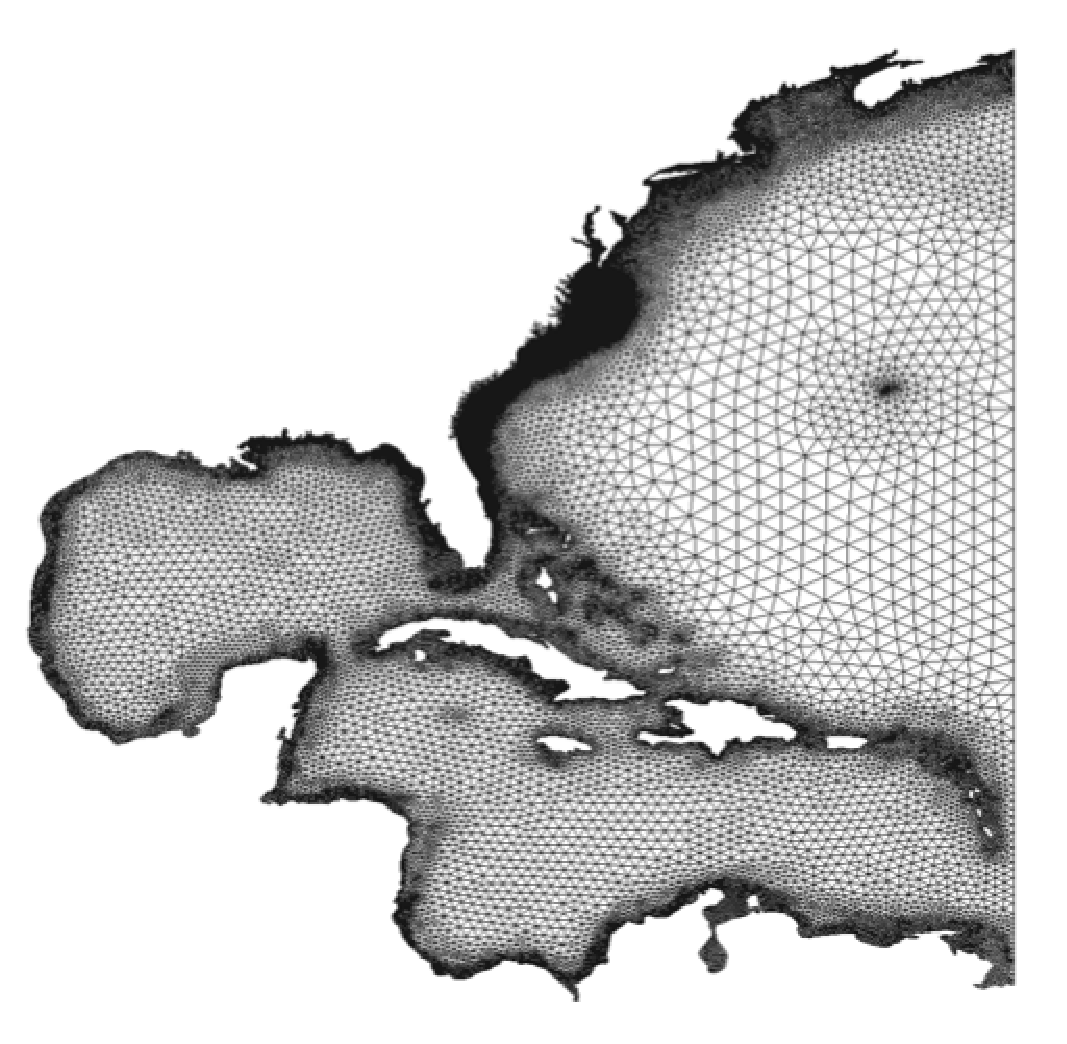
\includegraphics[width=0.5\textwidth]{ncv6b_mesh}\\
  \caption{North Carolina mesh.}
  \label{fig:nc_mesh}
\end{figure}

%    N C   B A T H Y
\begin{figure}[t]
  \centering
  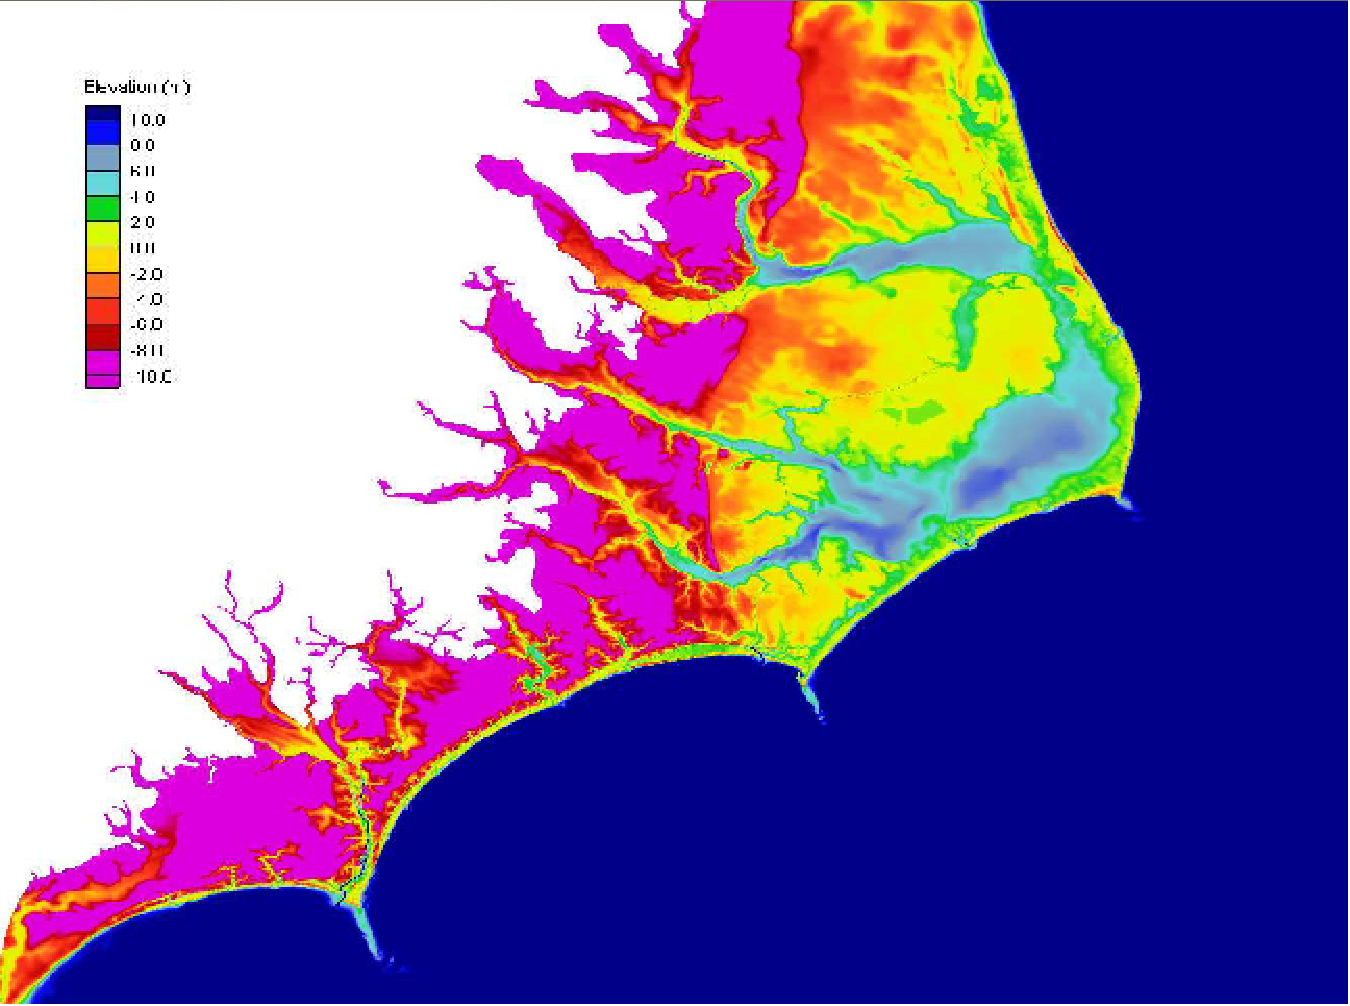
\includegraphics[width=0.5\textwidth]{ncv6b_bathy}\\
  \caption{North Carolina bathymetry.}
  \label{fig:nc_bathy}
\end{figure}

%    N C   L A N D C O V E R
\begin{figure}[t]
  \centering
  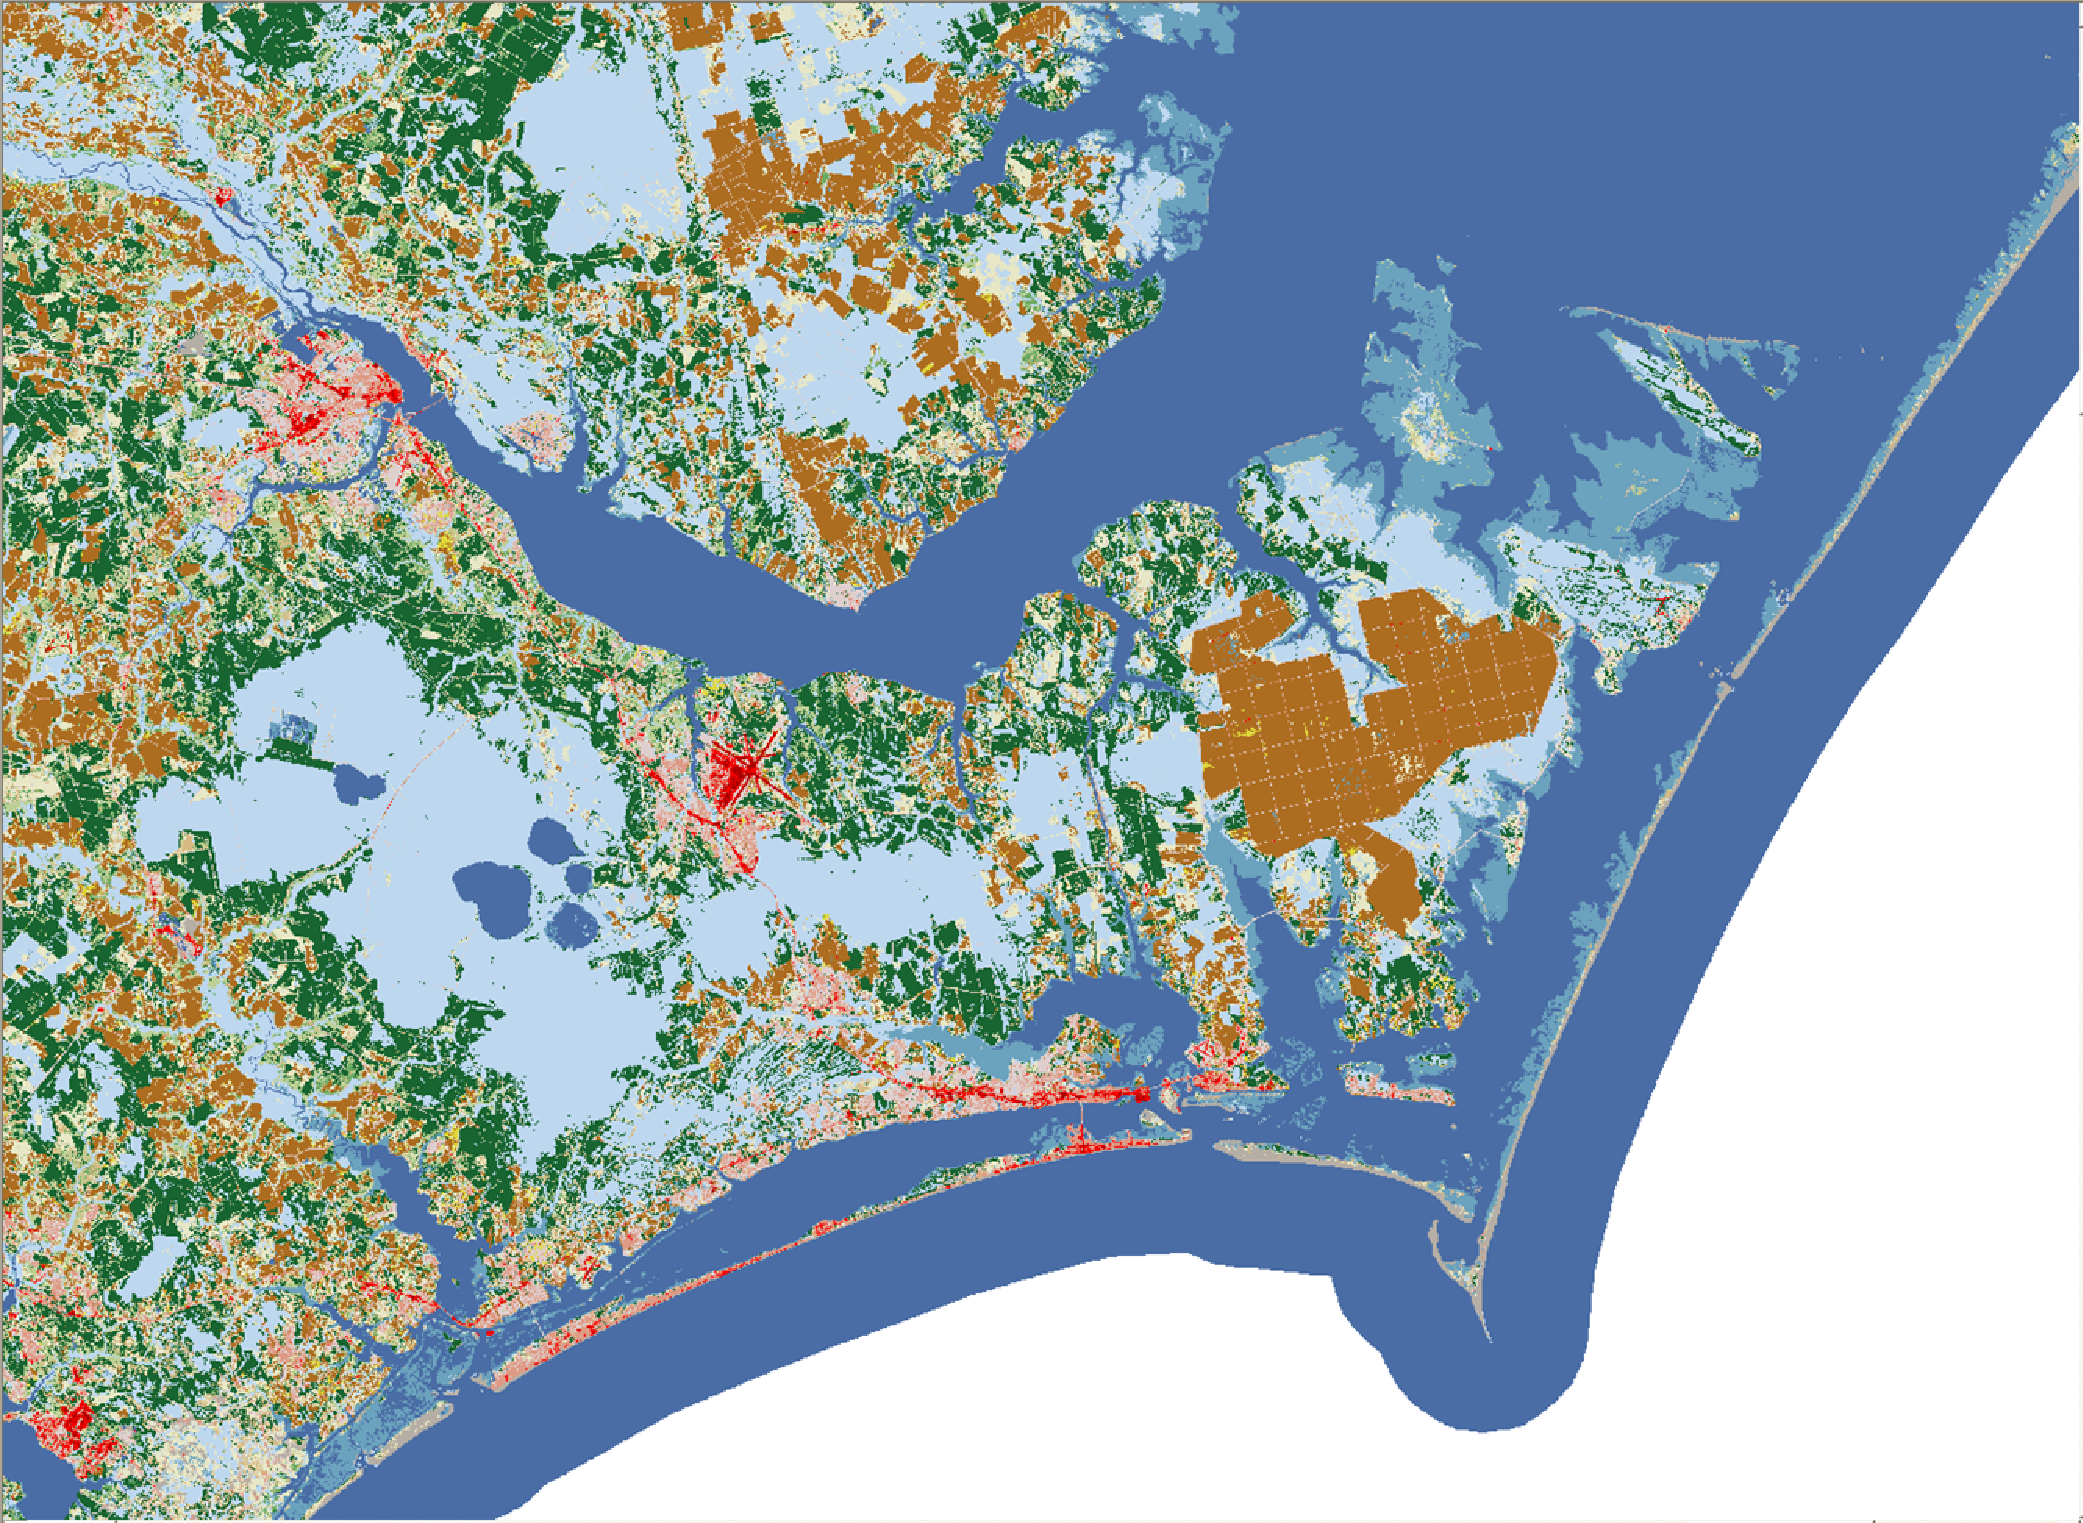
\includegraphics[width=0.5\textwidth]{nc_landcover}\\
  \caption{North Carolina land cover.}
  \label{fig:nc_landcover}
\end{figure}

%   S T O R M   P A R A M E T E R   V A R I A T I O N S
\begin{figure}[t]
  \centering
  \noindent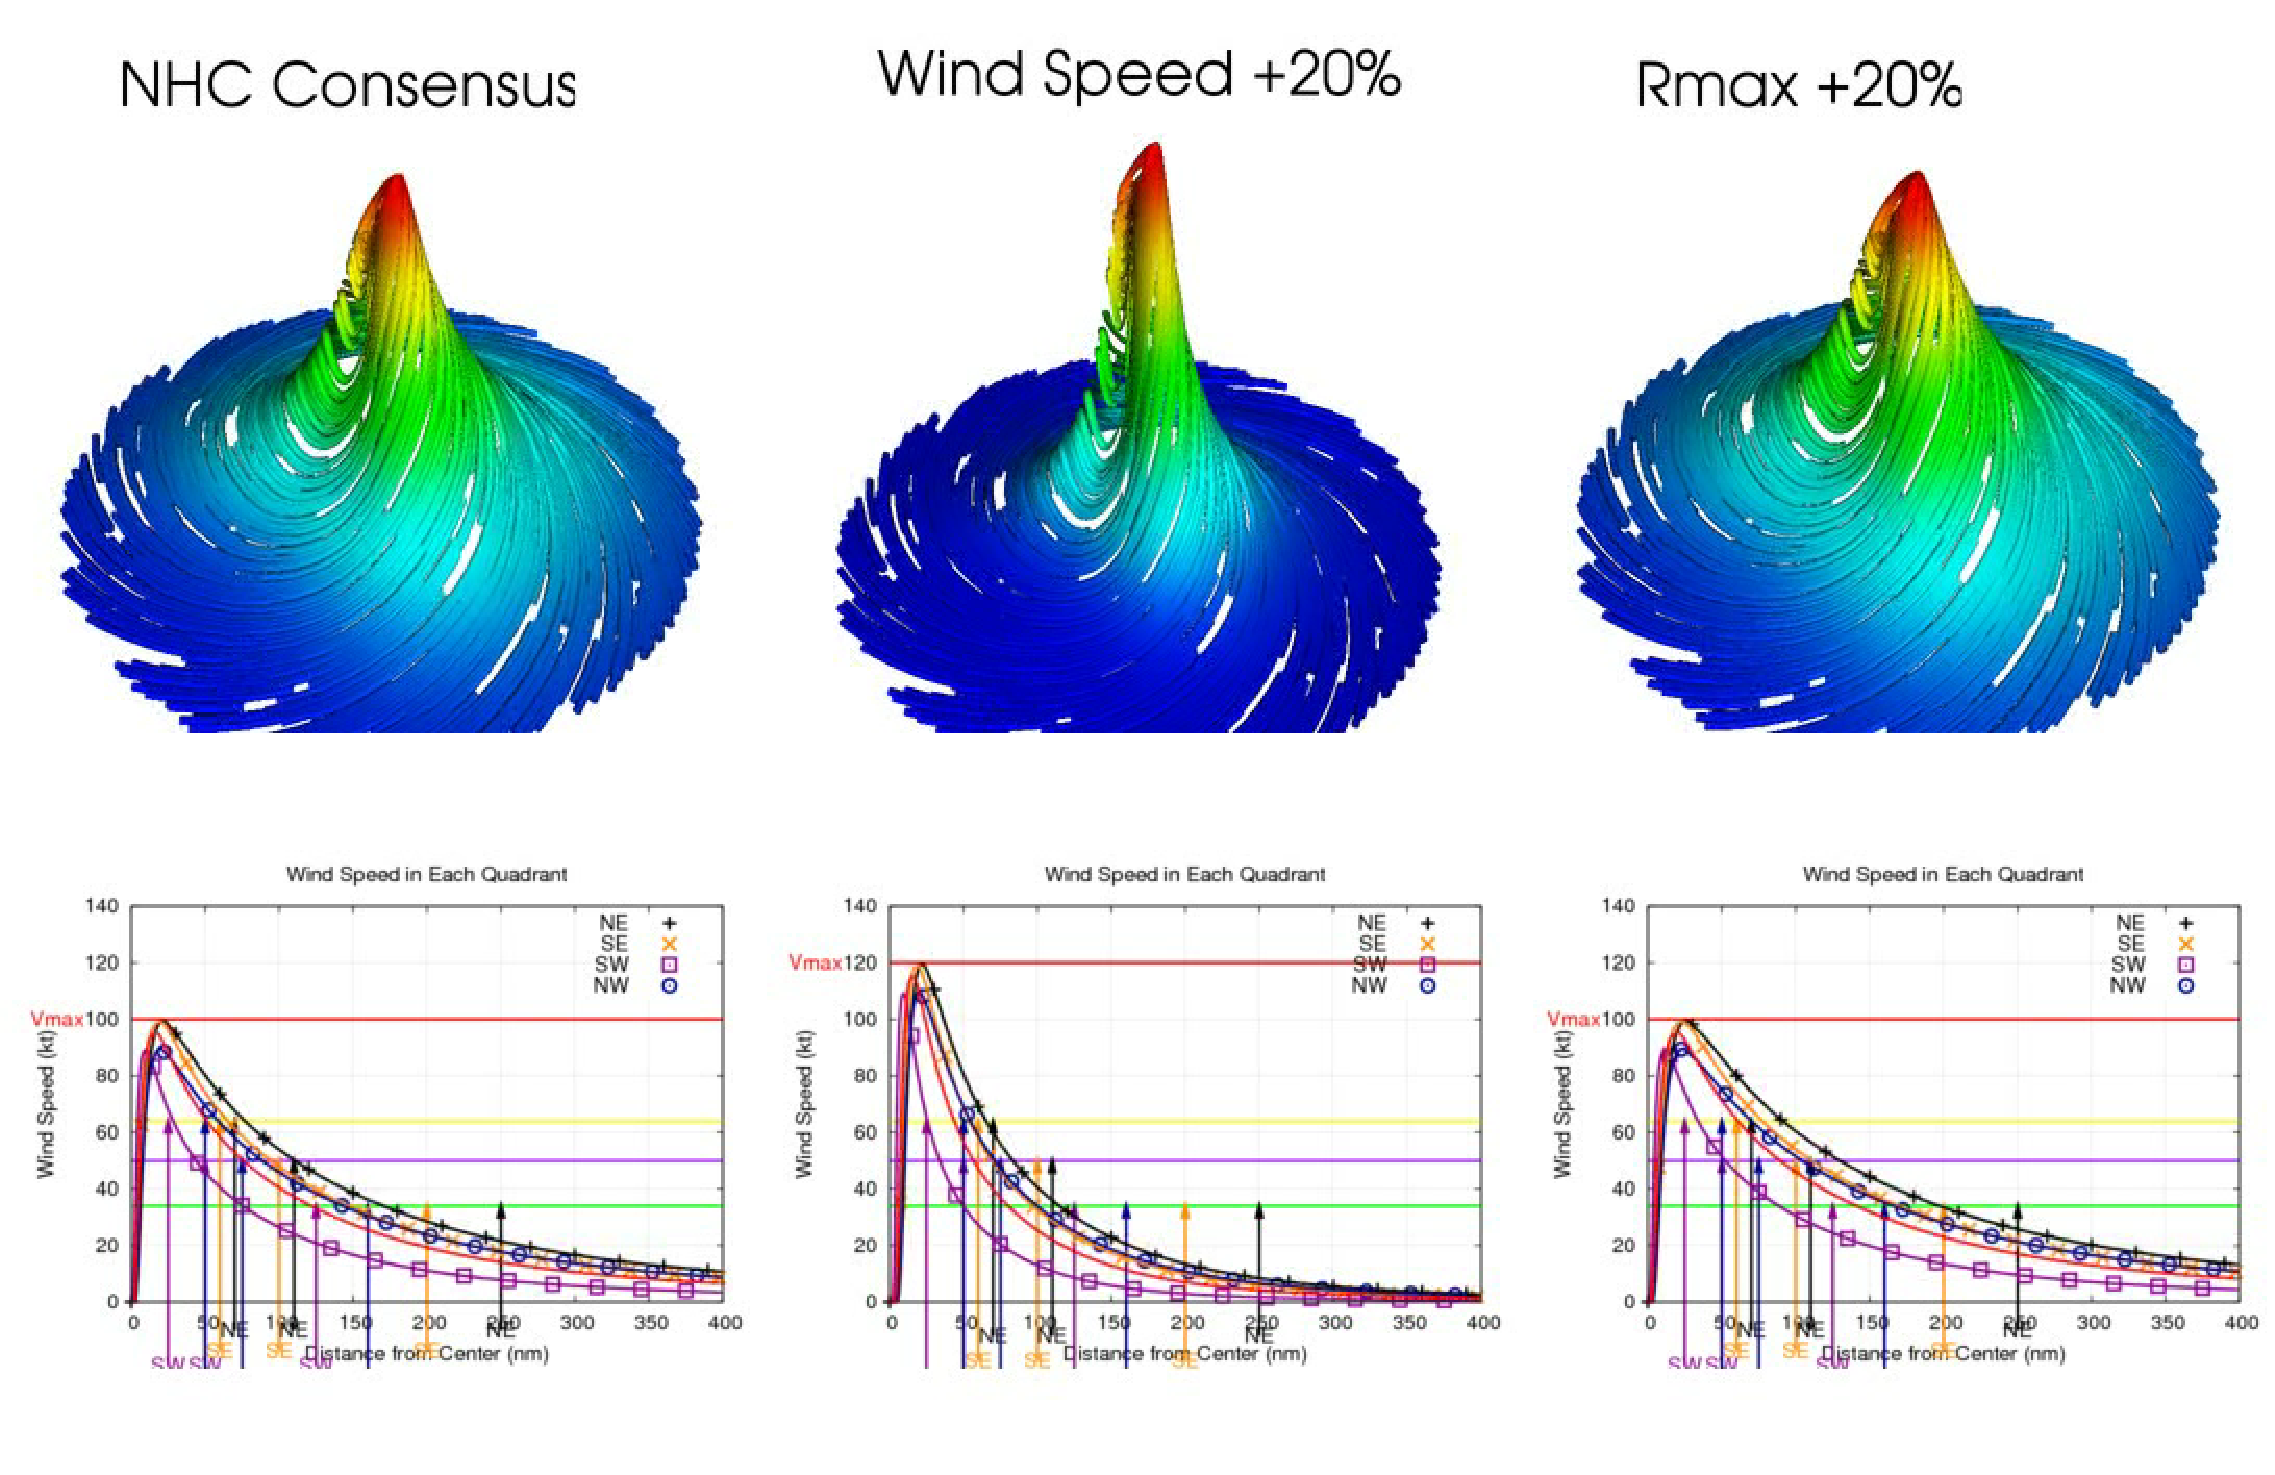
\includegraphics[width=0.5\textwidth]{variations}\\
  \caption{Storm variations.}
  \label{fig:storm_variations}
\end{figure}

%%%%%%%%%%%%%%%%%%%%%%%%%%%%%%%%%%%%%%%%%%%%%%%%%%%%%%%%%%
%%%%%%%%%%%%%%%%%%%%%%%%%%%%%%%%%%%%%%%%%%%%%%%%%%%%%%%%%%
\section{Results}

Implementation of the ASGS at the Renaissance Computing Institute 
(RENCI) in North Carolina, commonly referred to as the North 
Carolina Forecast System. (\cite{BlantonBO2012}). The NCFS downloads 
river flux boundary conditions for the Tar and Pamlico rivers; these 
boundary conditions are produced by a hydrological model operated by 
the National Severe Storms Lab and the University of Oklahoma (\cite
{VanCootenS2011}). 

During Hurricane Irene of 2011, the ASGS and CERA technologies were 
actively and heavily utilized by National Weather Service (NWS) 
offices, emergency managers, and the US Coast Guard. In one example 
of the real benefit for emergency management officials, US Coast 
Guard Admirals personally operated the web application to examine 
and interact with simulation results, and then used those results in 
their decision to evacuate their command center near Norfolk, VA, 
relocating to their secondary command center in Missouri. 
Subsequently, the predicted flooding did occur, rendering the 
abandoned USCG command center useless. In summary, the USCG was able 
to maintain uninterrupted command and control over the course of 
Hurricane Irene from their alternate command center, and have lauded 
the ASGS/CERA system for its contribution to this successful 
real time decision.

Hurricane Irene 2011 provided an oppportunity to use the ASGS and 
CERA technologies to assist officials in the NWS and USCG with 
real-life and emergency management decisions in real time. The 
implementation of these technologies for the North Carolina and US 
East Coast that provided the basis for this real life application 
are described below, including the static physical data, use of 
dynamic meteorological and river flow data, configuration, 
interaction with web-based results, and feedback from official end 
users. 

%{North Carolina Physical Data}

The discretization of the North Carolina domain (the mesh) that was 
used for both ADCIRC and SWAN is shown below in figure 3. The mesh 
contained 295328 nodes and 575512 with a minimum element size of 
13m. The land cover data that were used to derive directional wind 
roughness lengths, canopy coefficients, and Manning's n friction 
values are shown in figure 5. The system set 127 points throughout 
the domain for sampling the model output for comparison with tide 
gauges and water levels in river flood plains and other locations. 
It also specified 99 locations for point sampling of model 
meteorological data for comparison with physical meteorological data 
collected at land based and buoy-based meteorological data collected 
by various state and federal agencies and universities.

%{Dynamic Input Data}

As the storm that would eventually become Irene was forming, the 
ASGS/CERA system had already been running for months at RENCI on the 
blueridge machine, a 1408 core Dell High Performance Computing 
cluster, producing daily forecasts using NCEP NAM meteorology, river 
flow data from NSSL, and tidal forcing. 

When Irene formed and the decision was made to start running 
vortex-forced tropical cyclone forecasts, a new instance of the ASGS 
was started up from the most recent hotstart file from the existing 
NAM results. The new instance was configured to run on 384 
processors, rather than the 180 that were used in the NAM runs. Both 
ASGS instances then ran side by side for several days, sending their 
output to the CERA web application, until the NAM instance was shut 
down to conserve processor time.

%{Internally Generated Input Files}

On 384 processors, the ASGS was able to perform all file 
manipulations for the nowcast and forecast cycle for the consensus 
track, submit the jobs, and generate results for a 5 day forecast in 
1 hour 15 minutes from the time the NHC forecast/advisory was issued. 

As hurricane Irene approached the North Carolina coast, the team 
member that operates of the ASGS system lost electric power and 
could therefore no longer oversee the operation of the ASGS during 
this critical period. However, since the ASGS itself was actually 
executing at the RENCI facility, which is located in Durham, North 
Carolina and that facility never lost power, the ASGS was able to 
continue operating autonomously without interruption and without 
interaction or oversight for the duration of the storm.  

%{Output Visualization and Interaction}

The results produced by the ASGS were converted in-situ to Google 
Earth (kmz) graphics and posted to the OpenDAP server at RENCI for 
use by the Newport NWS forecast office. The raw data in NetCDF 
format were also posted to the OpenDAP server and then a 
notification email was sent to the CERA web application. 

The web application picked up the latest raw data, generated the 
image tiles for the animations and maximum values visualizations at 
all levels of detail, and sent email notification to selected 
official end users at NOAA and the USCG to notify them that new 
results were available for interaction over the web. The CERA 
website itself was not password protected, but end users were 
instructed not to publicize the availability of the site. The CERA 
web processing required another 1 hour and 15 minutes to generate 
image tiles for a particular advisory, for a total turn around time 
of 2 hours and 30 minutes.

There were myriad examples of the use of the ASGS/CERA results by 
emergency managers and officials during the storm event. As stated 
in the executive summary, several Admirals at the USCG personally 
examined and interacted with the ASGS/CERA results via the CERA site 
and subsequently made the real time decision to evacuate their 
command center in Virginia. The flooding depicted in the results did 
occur, and the USCG was extremely pleased and satisfied with their 
experience with the ASGS/CERA guidance.

\section{Conclusions}

What does it all mean?

%%%%%%%%%%%%%%%%%%%%%%%%%%%%%%%%%%%%%%%%%%
%%%%%%%%%%%%%%%%%%%%%%%%%%%%%%%%%%%%%%%%%%

\acknowledgements{Acknowledgements}

This material is based upon work supported by the US Army Corps of 
Engineers, New Orleans District, under Award Numbers: 
W912P8-09-P-0324 and W912P8-13-C-0036; the Coastal Hazards Center of 
Excellence, a US Department of Homeland Security Science and 
Technology Center of Excellence under Award Number: 2008-ST-061-ND 
0001; and the University of North Carolina at Chapel Hill 
Renaissance Computing Institute. Disclaimer: The views and 
conclusions contained in this document are those of the authors and 
should not be interpreted as necessarily representing the official 
policies, either expressed or implied, of the US Department of 
Homeland Security.

%%%%%%%%%%%%%%%%%%%%%%%%%%%%%%%%%%%%%%%%%%

\conflictofinterests{Conflicts of Interest}

The authors declare no conflicts of interest. 

%=================================================================
% References: Variant A
%=================================================================
% Back Matter (References and Notes)
%----------------------------------------------------------
% Style and layout of the references
%\bibliographystyle{mdpi}
%\makeatletter
%\renewcommand\@biblabel[1]{#1. }
%\makeatother

%\begin{thebibliography}{1}

% Reference 1
%\bibitem{ref-journal}
%Lastname, F.; Author, T. The title of the cited article. {\em Journal Abbreviation} {\bf 2008}, {\em 10}, 142-149.

% Reference 2
%\bibitem{ref-book}
%Lastname, F.F.; Author, T. The title of the cited contribution. In {\em The Book Title}; Editor, F., Meditor, A., Eds.; Publishing House: City, Country, 2007; pp. 32-58.

%\end{thebibliography}

%=================================================================
% References:  Variant B
%=================================================================
% Use the following option to include external BibTeX files:
\bibliography{references}
\bibliographystyle{mdpi}



\end{document}

